% !TeX program = pdflatex
\documentclass[11pt,a4paper]{article}
\usepackage[utf8]{inputenc}
\usepackage[T1]{fontenc}
\usepackage[spanish,es-nodecimaldot]{babel}
\usepackage[margin=1.7cm]{geometry}
\usepackage{lmodern,graphicx,float,caption,parskip,tabularx,booktabs,array,enumitem}
\usepackage[hidelinks]{hyperref}
\graphicspath{{imagenes/}}
\captionsetup{font=small,labelfont=bf}
\setlength{\parskip}{5pt}\setlength{\intextsep}{4pt}\setlength{\emergencystretch}{4em}
\newcolumntype{Y}{>{\raggedright\arraybackslash}X}
\newcolumntype{P}[1]{>{\raggedright\arraybackslash}p{#1}}
\setlist[enumerate]{leftmargin=*,itemsep=3pt}
\title{\vspace{-1.5cm}Auditoría de una infraestructura\\industrial simulada}
\author{Lorenzo\\Universidad Santo Tomás -- Ciberseguridad en la Industria}
\date{Demostración práctica: 17 de noviembre de 2026}
\begin{document}\maketitle\vspace{-0.8cm}
\section*{1. Diagrama de la infraestructura virtual implementada}\label{infraestructura}
El laboratorio reúne una máquina de auditoría Kali, una víctima Metasploitable 2 y un Ubuntu con ModbusPal, que simula la comunicación de un PLC (controlador lógico programable). Se utilizó la red aislada \texttt{192.168.212.0/24}; Windows también pertenece a ella como anfitrión.
\begin{figure}[H]\centering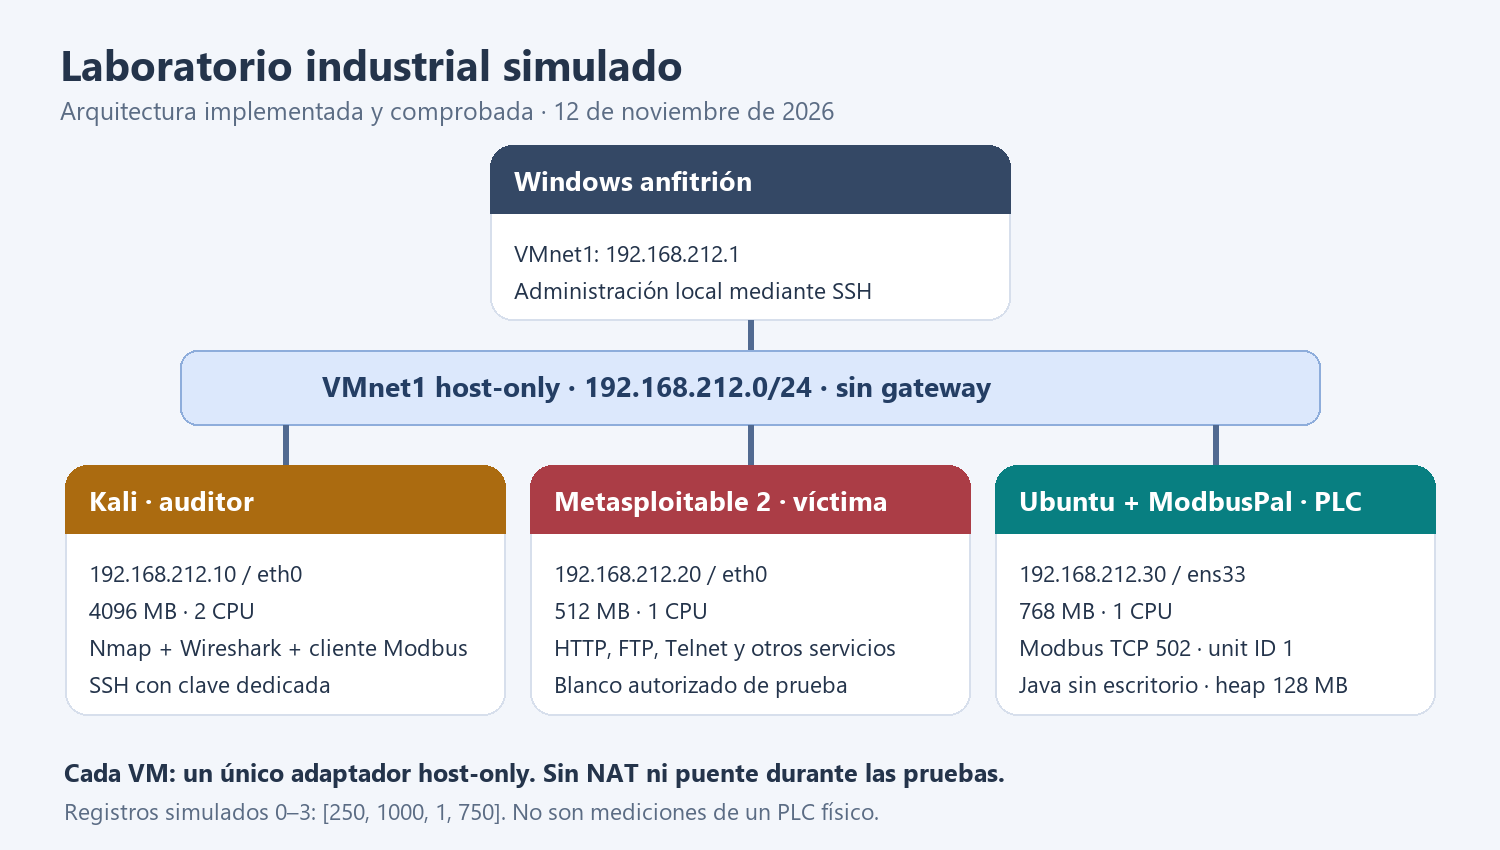
\includegraphics[width=0.95\linewidth]{arquitectura.png}\caption{Roles, direcciones y recursos del montaje.}\end{figure}
\textbf{Lectura del esquema.} Kali origina las consultas; Metasploitable responde con sus servicios de prueba; ModbusPal mantiene cuatro registros industriales simulados. Las IP identifican las máquinas; los puertos distinguen servicios dentro de cada una. No se utilizaron dispositivos físicos de producción.
\textbf{Montaje.} Se reutilizó Kali (4 GB y 2 CPU), se importó Metasploitable 2 (512 MB y 1 CPU) y se preparó Ubuntu/ModbusPal (768 MB y 1 CPU). Cada invitado quedó con un adaptador host-only, direcciones fijas y sin gateway. Se habilitó SSH (Secure Shell) para administración cifrada. El PLC limpio recibió paquetes antes de quedar aislado.

\clearpage\section*{1. Infraestructura: comprobación antes de las pruebas}\label{red}

\textbf{1. Encender y comprobar las máquinas.} Se revisó que solo estuvieran conectadas a la red del laboratorio. Al arrancar Kali se detectó reenvío IP activo y se desactivó antes de sondear. Conviene repetir esta comprobación al preparar la sustentación.

\begin{quote}\ttfamily\small\raggedright ip -br address; ip route; sysctl net.ipv4.ip\_forward net.ipv6.conf.all.forwarding\par\end{quote}

\begin{figure}[H]\centering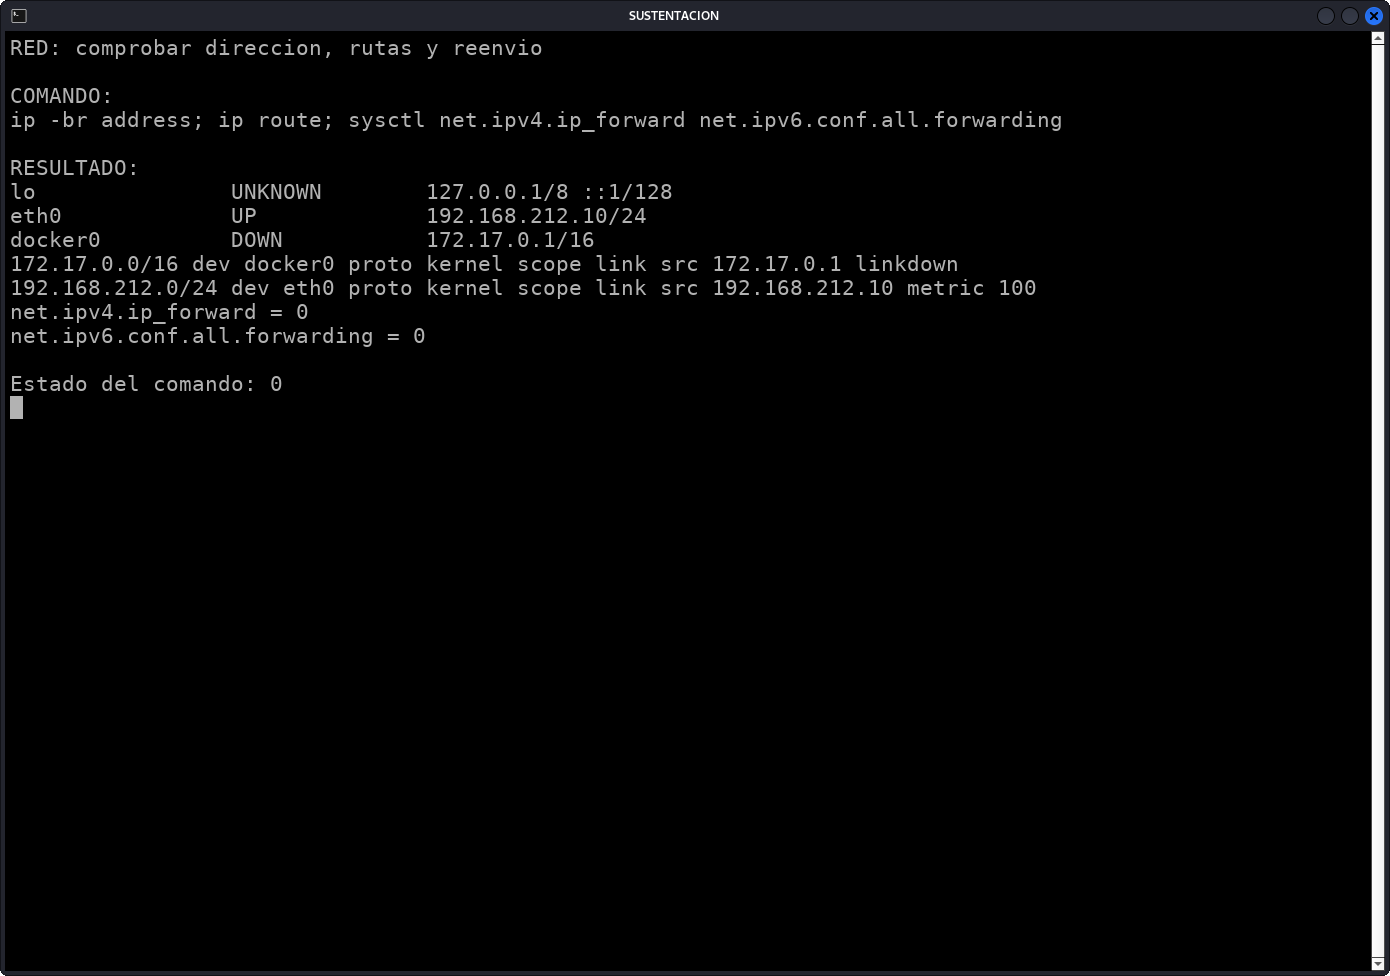
\includegraphics[width=1.0\linewidth,trim=0 534bp 0 0,clip]{sustentacion/01-estado.png}\caption{Dirección de Kali, rutas y reenvío después de preparar la red.}\end{figure}

\textbf{Qué se observa.} \texttt{eth0} tiene \texttt{192.168.212.10/24}; la ruta al laboratorio es directa y no aparece una ruta \texttt{default}. Los valores de reenvío son 0: Kali no transporta tráfico entre redes. \texttt{docker0} permanece inactivo y no participa en las pruebas.
\textbf{2. Comprobar el PLC.} El servicio \texttt{modbuspal-lab} respondió en \texttt{.30:502}. Los registros configurados fueron \texttt{[250,1000,1,750]}. Son enteros de prueba, sin unidades físicas asignadas. La lectura y su evidencia se presentan en el análisis de comunicaciones.

\clearpage\section*{2. Tabla de dispositivos, direcciones IP, puertos y servicios}\label{tabla}

Todos los puertos inventariados son TCP (Transmission Control Protocol), el transporte que ordena y entrega bytes entre dos extremos. TCP no cifra por sí mismo. Un extremo combina una dirección IP (Internet Protocol) y un número de puerto.
{\small\renewcommand{\arraystretch}{1.15}
\par\begin{tabularx}{\linewidth}{@{}P{2.8cm}P{2.8cm}P{2.5cm}Y@{}}\toprule
Dispositivo & IP & Puertos & Servicios y función\\\midrule
Windows & 192.168.212.1 & No sondeados & Administración de la red virtual.\\
Kali & 192.168.212.10 & 22 verificado por SSH & Auditor; Nmap, Wireshark y clientes HTTP/Modbus/Telnet.\\
Metasploitable 2 & 192.168.212.20 & Inventario inferior & Víctima autorizada; servicios identificados con Nmap.\\
Ubuntu + ModbusPal & 192.168.212.30 & 22 y 502 & SSH y Modbus TCP confirmado por lectura FC03.\\\bottomrule
\end{tabularx}}
\textbf{Detalle de la víctima.} Se exploraron sus 65.535 puertos TCP. En el PLC se examinaron únicamente 22 y 502; no se realizó inventario UDP ni sondeo de puertos del anfitrión o de Kali.
{\fontsize{9}{10.5}\selectfont\setlength{\tabcolsep}{3pt}\par\begin{tabularx}{\linewidth}{rYrY}\toprule
Puerto & Servicio / versión & Puerto & Servicio / versión\\\midrule

21 & ftp / vsftpd 2.3.4 & 2121 & ftp / ProFTPD 1.3.1\\

22 & ssh / OpenSSH 4.7p1 Debian 8ubuntu1 protocol 2.0 & 3306 & mysql / MySQL 5.0.51a-3ubuntu5\\

23 & telnet / Linux telnetd & 3632 & distccd / distccd v1 (GNU) 4.2.4 (Ubuntu 4.2.4-1ubuntu4)\\

25 & smtp / Postfix smtpd & 5432 & postgresql / PostgreSQL DB 8.3.0 - 8.3.7\\

53 & domain / ISC BIND 9.4.2 & 5900 & vnc / VNC  protocol 3.3\\

80 & http / Apache httpd 2.2.8 (Ubuntu) DAV/2 & 6000 & X11 / access denied\\

111 & rpcbind & 6667 & irc / UnrealIRCd\\

139 & netbios-ssn / Samba smbd 3.X - 4.X workgroup: WORKGROUP & 6697 & irc / UnrealIRCd  Admin email admin@Metasploitable.LAN\\

445 & netbios-ssn / Samba smbd 3.0.20-Debian workgroup: WORKGROUP & 8009 & ajp13 / Apache Jserv  Protocol v1.3\\

512 & exec / netkit-rsh rexecd & 8180 & unknown\\

513 & login & 8787 & drb / Ruby DRb RMI  Ruby 1.8; path /usr/lib/ruby/1.8/drb\\

514 & shell / Netkit rshd & 41128 & unknown\\

1099 & java-rmi / GNU Classpath grmiregistry & 44426 & unknown\\

1524 & bindshell / Metasploitable root shell & 45634 & unknown\\

2049 & rpcbind & 54652 & unknown\\

\bottomrule\end{tabularx}}
Se conservan las identificaciones inciertas de Nmap. Una versión o un puerto abierto orienta la investigación, pero no confirma por sí solo una vulnerabilidad explotada.

\clearpage\section*{3. Evidencias del reconocimiento realizado con Nmap}\label{nmap1}

\par\textbf{1. Descubrir los blancos.} Nmap envía consultas a las dos direcciones autorizadas para comprobar si responden. \texttt{-sn} hace descubrimiento, sin inventariar todos los puertos; \texttt{-oA} conserva los resultados en varios formatos.
\begin{figure}[H]\centering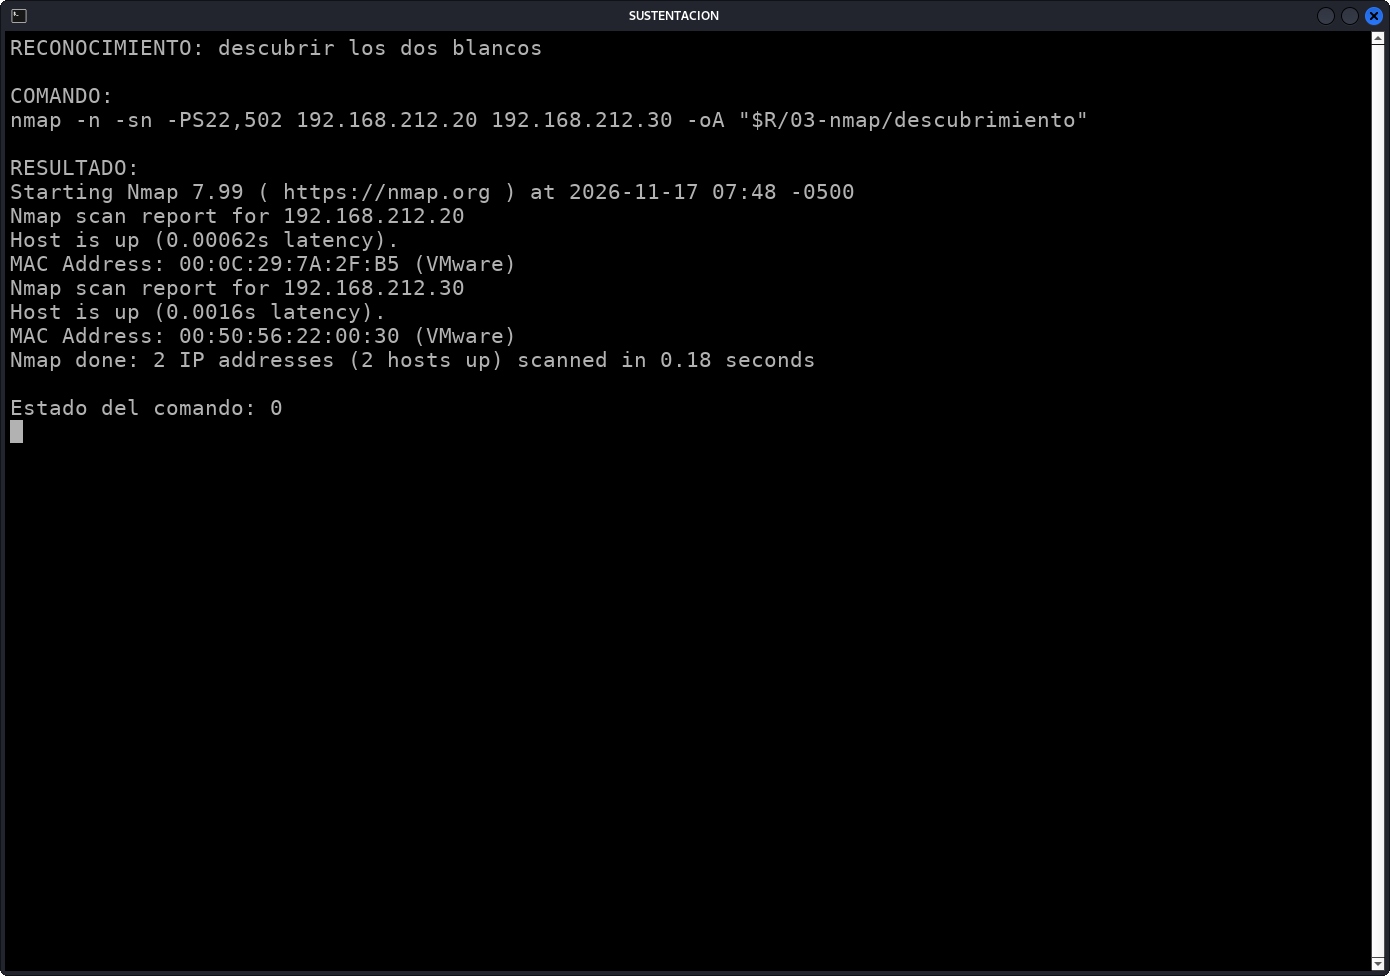
\includegraphics[width=1.0\linewidth,trim=0 510bp 0 0,clip]{sustentacion/02-descubrimiento.png}\caption{Consulta de descubrimiento y respuesta de los dos equipos.}\end{figure}

\par\textbf{Lectura.} Cada bloque \texttt{Nmap scan report} identifica una IP; \texttt{Host is up} confirma respuesta. La MAC es el identificador de la tarjeta de red dentro del enlace virtual.
\par\textbf{2. Sondear la víctima.} Se utilizó \texttt{-sT} para conexiones TCP, \texttt{-sV} para detectar servicios/versiones, \texttt{-sC} para scripts predeterminados y \texttt{-p-} para todos los puertos TCP. La salida completa quedó conservada; la vista siguiente reúne las filas de puertos.
\begin{quote}\ttfamily\small\raggedright nmap -n -sT -sV -sC --version-light --script-timeout 30s --host-timeout 600s -p- 192.168.212.20 -oA "\$R/03-nmap/metasploitable"\par\end{quote}

\begin{figure}[H]\centering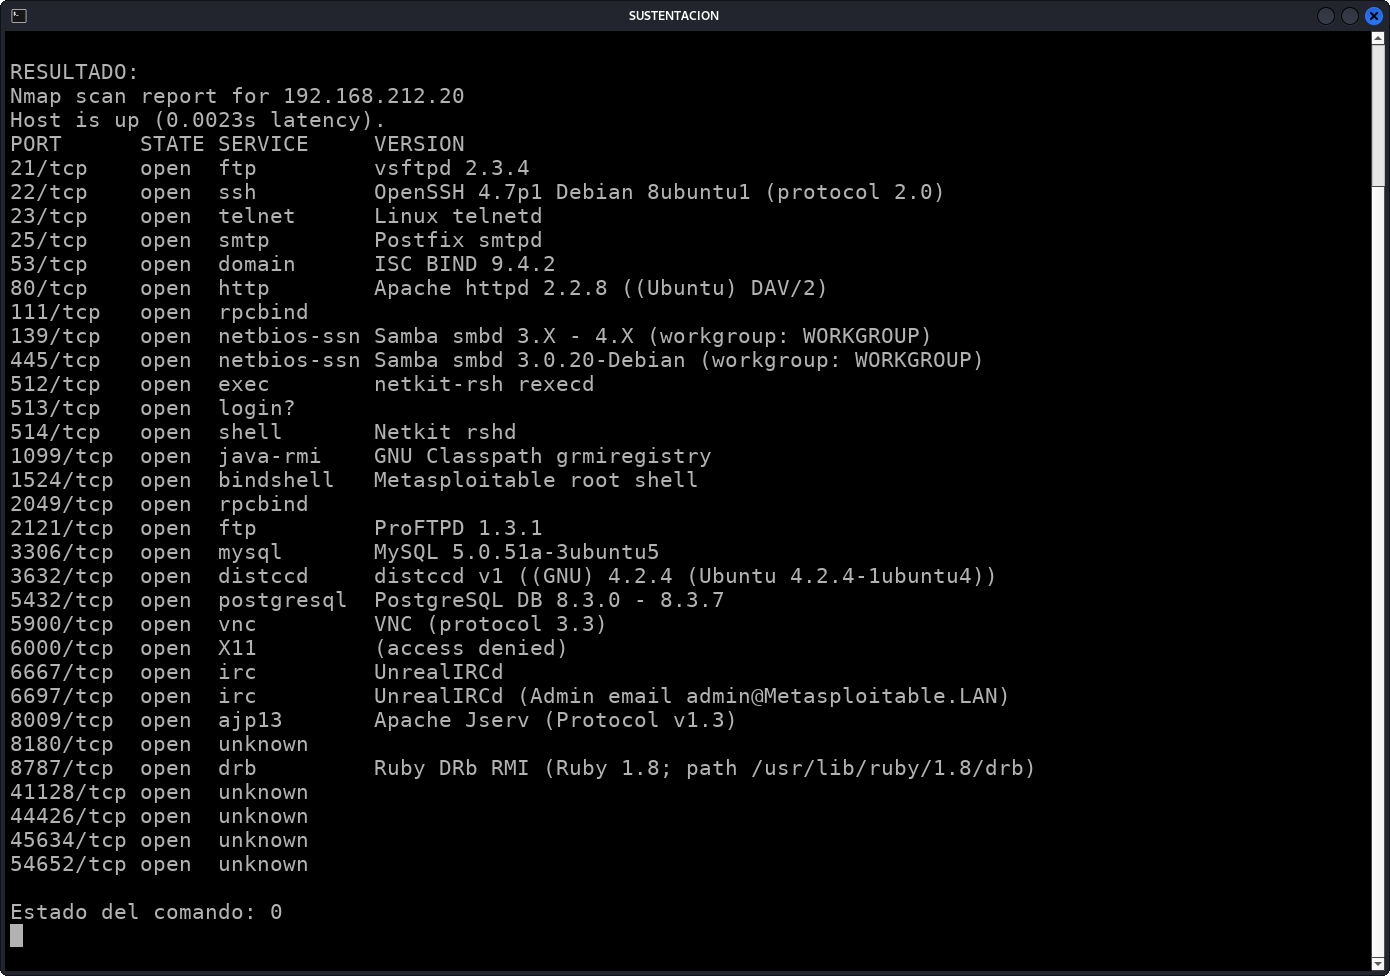
\includegraphics[width=0.92\linewidth,trim=0 6bp 0 0,clip]{sustentacion/03-nmap-victima.png}\caption{Servicios identificados en el sondeo completo de Metasploitable 2.}\end{figure}

\clearpage\section*{3. Reconocimiento: comprobar el servicio industrial}\label{nmap2}

\par\textbf{3. Sondear el PLC.} La consulta se limitó a 22 y 502. El primero corresponde a administración SSH; el segundo es el puerto del simulador industrial.
\begin{figure}[H]\centering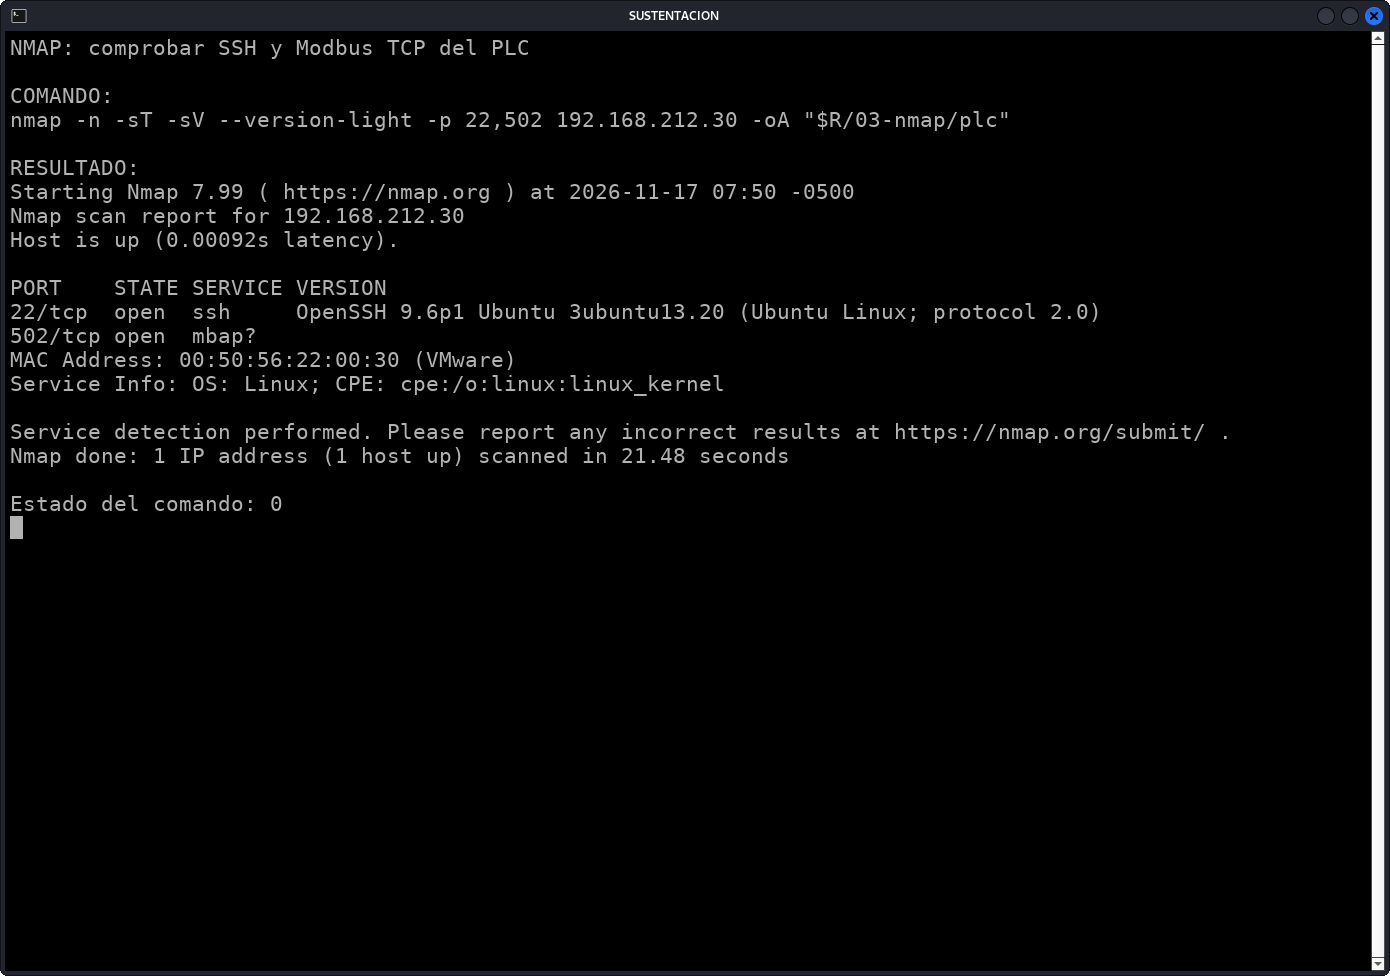
\includegraphics[width=1.0\linewidth,trim=0 414bp 0 0,clip]{sustentacion/04-nmap-plc.png}\caption{Puertos examinados en el Ubuntu que ejecuta ModbusPal.}\end{figure}

\par\textbf{Interpretación.} \texttt{open} significa que el destino acepta la conexión. La etiqueta de detección en 502 puede ser incierta; la lectura válida de registros que se muestra después confirma Modbus TCP. Los archivos XML y NMAP permiten volver a consultar el inventario sin repetir el sondeo.
\par\textbf{Cómo presentarlo.} Mostrar primero los equipos activos, después la tabla de servicios y señalar Telnet, HTTP y Modbus como los servicios que se utilizarán en los pasos siguientes. Mantener el sondeo limitado a las direcciones del laboratorio.
\clearpage\section*{4. Capturas y análisis del tráfico en Wireshark}\label{captura}

\textbf{Qué se conserva.} PCAP significa Packet Capture: un archivo de tráfico. Aquí se utiliza el formato PCAPNG, Packet Capture Next Generation. No es una imagen: contiene bytes y metadatos. Dumpcap registra la red; Wireshark permite abrir el archivo y analizarlo; TShark consulta los mismos datos desde la terminal. Una trama es un registro numerado de la captura y se muestra como una fila en Wireshark.
\textbf{1. Capturar antes de generar tráfico.} Se registró \texttt{eth0} durante 90 segundos. El filtro limita los datos a la víctima y el PLC; la orden se inició en segundo plano para poder lanzar las consultas.

\begin{figure}[H]\centering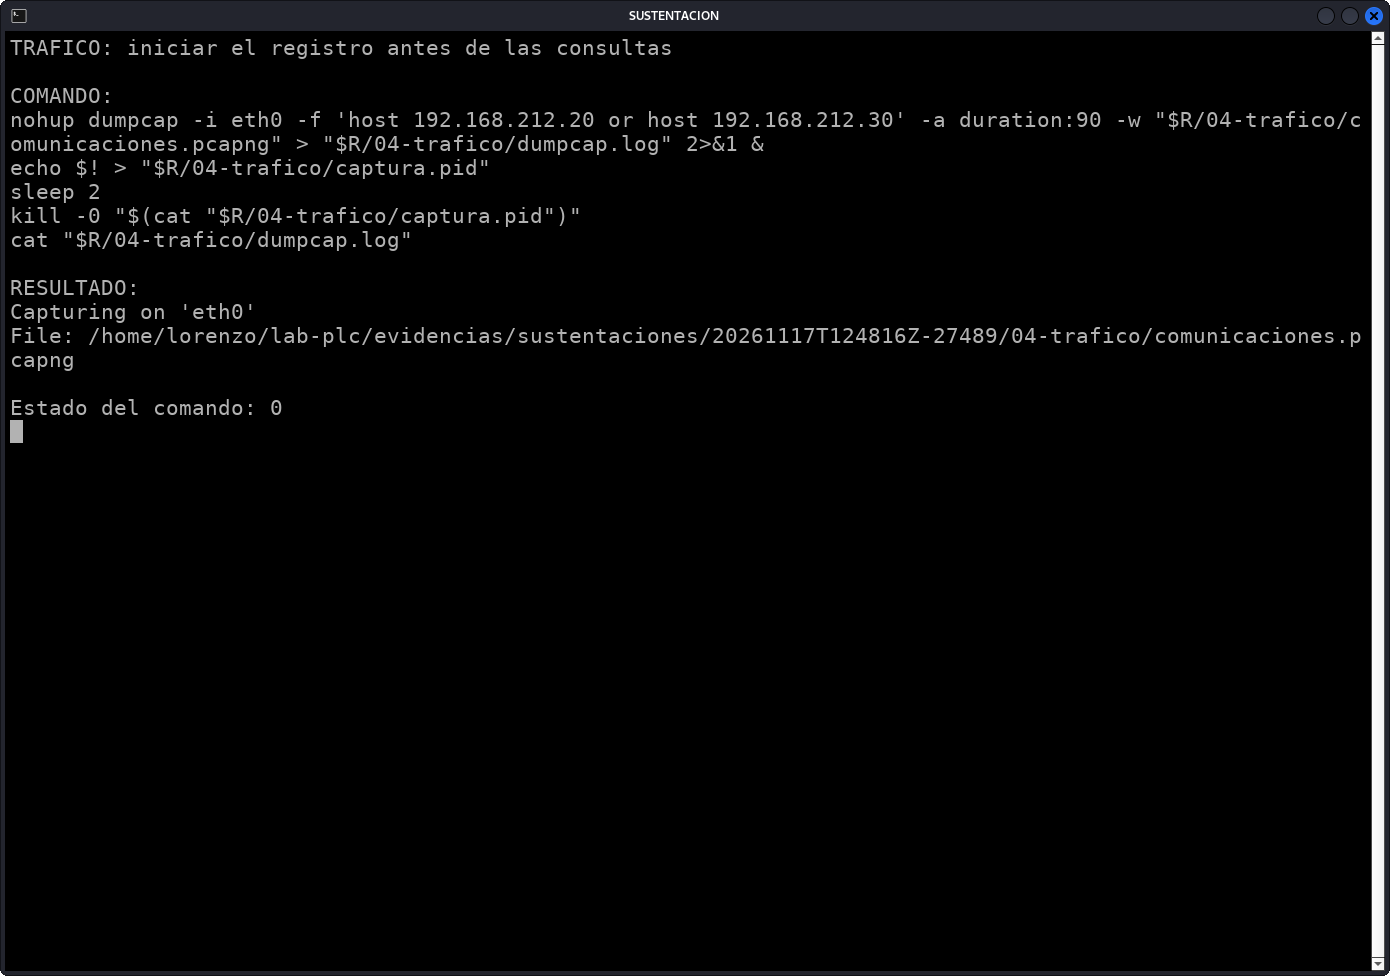
\includegraphics[width=1.0\linewidth,trim=0 510bp 0 0,clip]{sustentacion/05-inicio-captura.png}\caption{Inicio de dumpcap y comprobación de que el proceso sigue activo.}\end{figure}

\par\textbf{2. Solicitar una página.} curl es un cliente de terminal. La orden pidió la página principal de la víctima y guardó el cuerpo y los encabezados HTTP (Hypertext Transfer Protocol).
\begin{figure}[H]\centering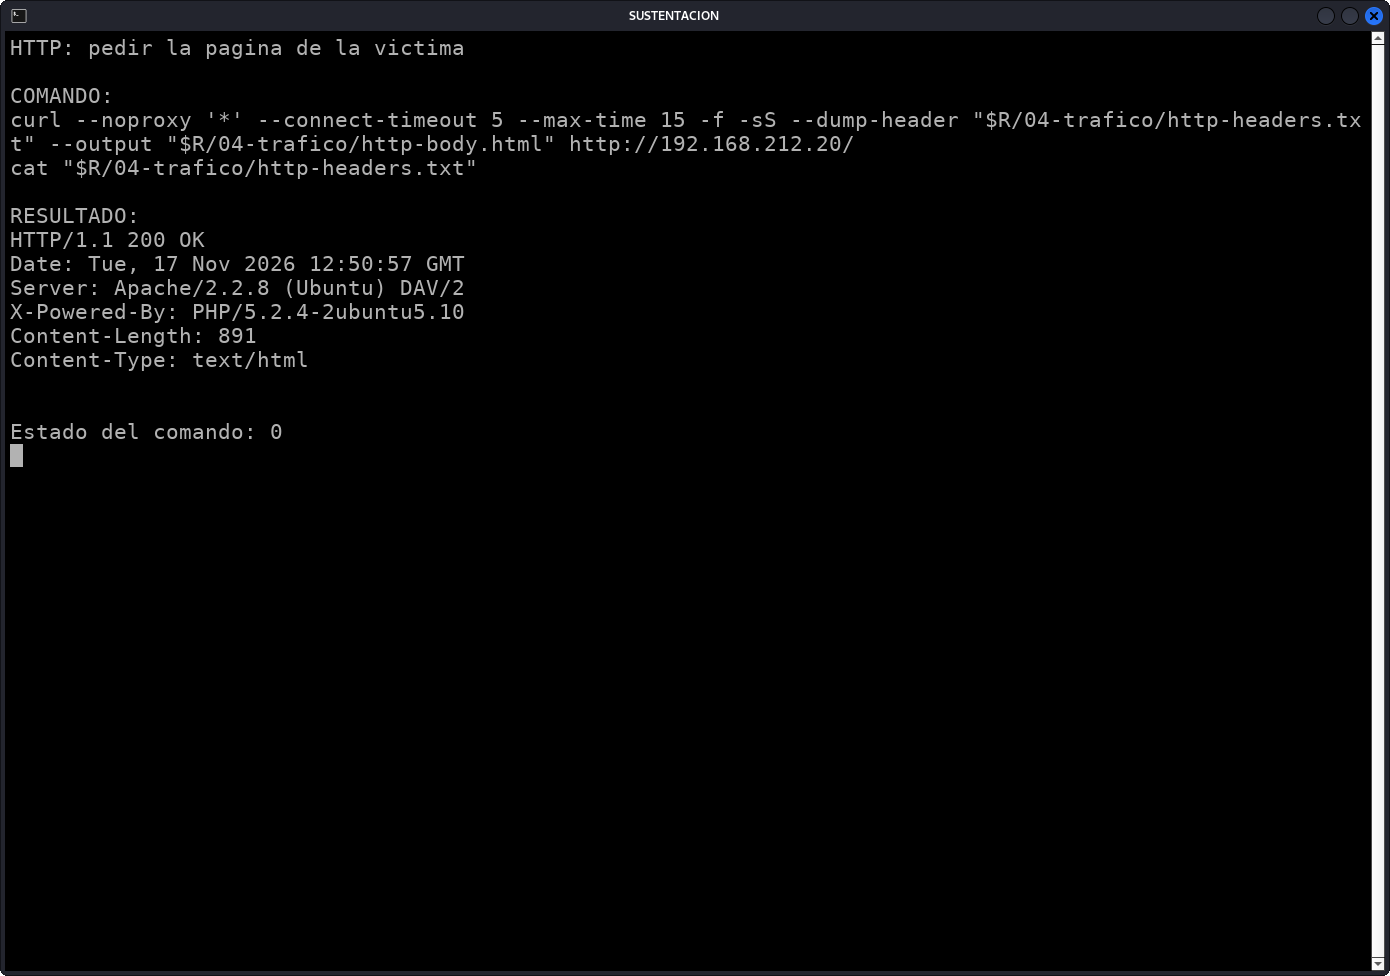
\includegraphics[width=1.0\linewidth,trim=0 486bp 0 0,clip]{sustentacion/06-http.png}\caption{Solicitud web y encabezados devueltos por el servidor.}\end{figure}

\par\textbf{Lectura.} \texttt{200 OK} indica que el servidor atendió la petición. Esta consulta genera los mensajes que después se reconocen en Wireshark.
\clearpage\section*{4. Tráfico: generar la lectura Modbus}\label{modbus-consulta}

\par\textbf{3. Consultar el PLC simulado.} El cliente se dirigió a \texttt{.30:502}, unidad 1. \texttt{--address 0 --count 4} significa empezar en el primer registro solicitado y leer cuatro. FC03 es la función Modbus para leer registros de almacenamiento de 16 bits.
\begin{figure}[H]\centering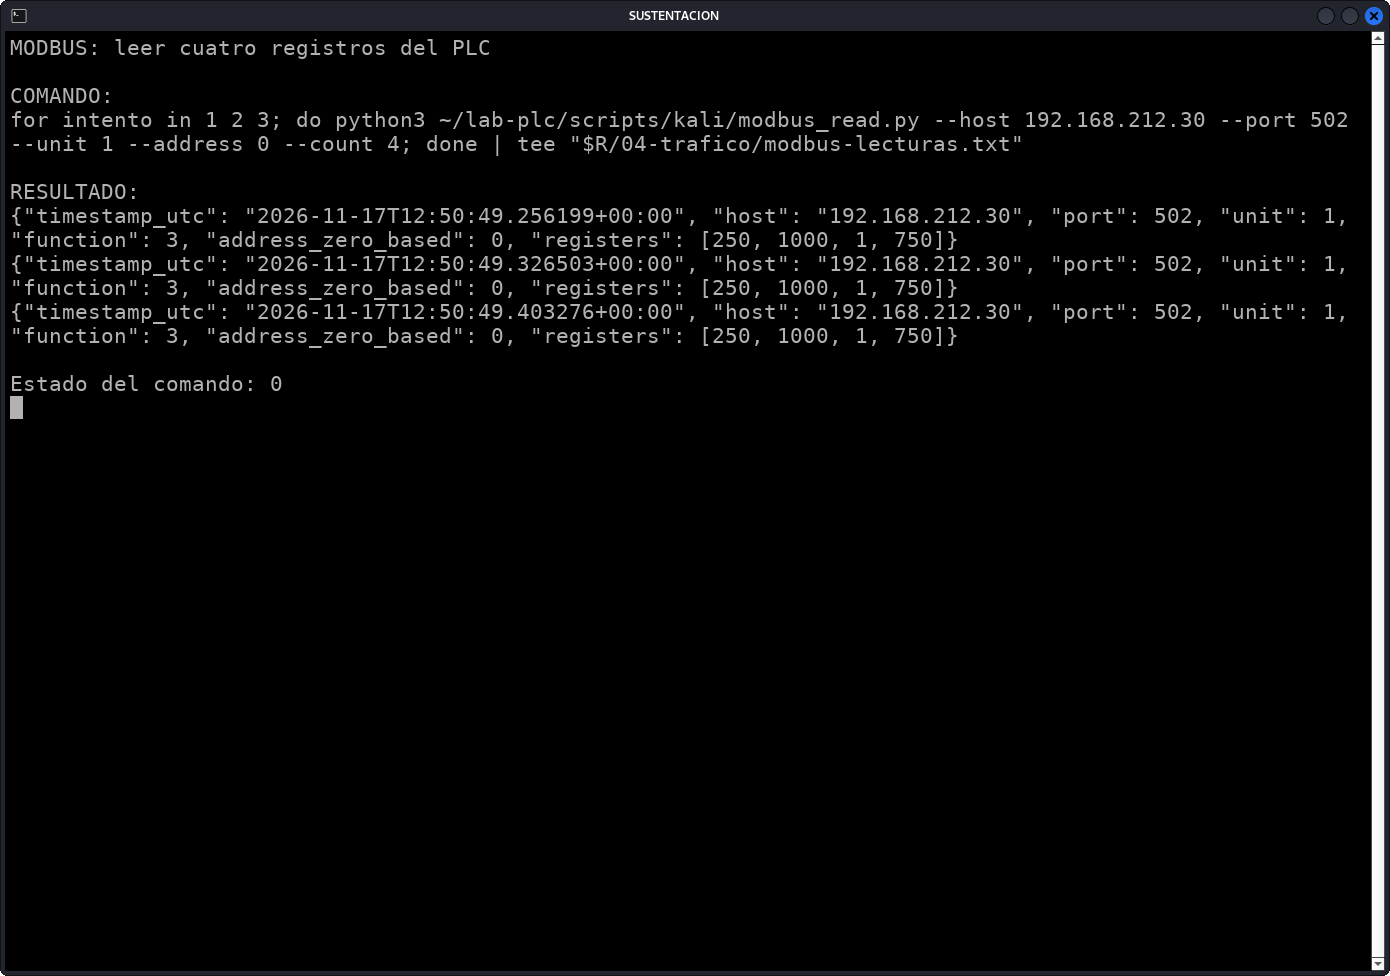
\includegraphics[width=1.0\linewidth,trim=0 534bp 0 0,clip]{sustentacion/07-modbus.png}\caption{Tres consultas reales y valores devueltos por ModbusPal.}\end{figure}

\par\textbf{Lectura.} Cada resultado identifica el destino, el puerto, la unidad, la función y el arreglo \texttt{registers}. Las tres respuestas deben mostrar \texttt{[250,1000,1,750]}. No se envió una orden de escritura. Se esperó el cierre de la captura antes del análisis.
\par\textbf{Orden para exponer.} Iniciar captura, solicitar HTTP, leer Modbus, esperar el cierre y abrir el PCAP. Conservar la terminal abierta mantiene la variable \texttt{R}, que señala la carpeta de la corrida.
\clearpage\section*{4. Tráfico: reconocer el establecimiento TCP}\label{tcp}

\par\textbf{4. Localizar el inicio de la conversación.} Las primeras tres tramas de la conexión HTTP son 1, 2, 3. SYN solicita conectar; SYN-ACK acepta y reconoce; ACK confirma. Después puede circular la petición web.
\begin{figure}[H]\centering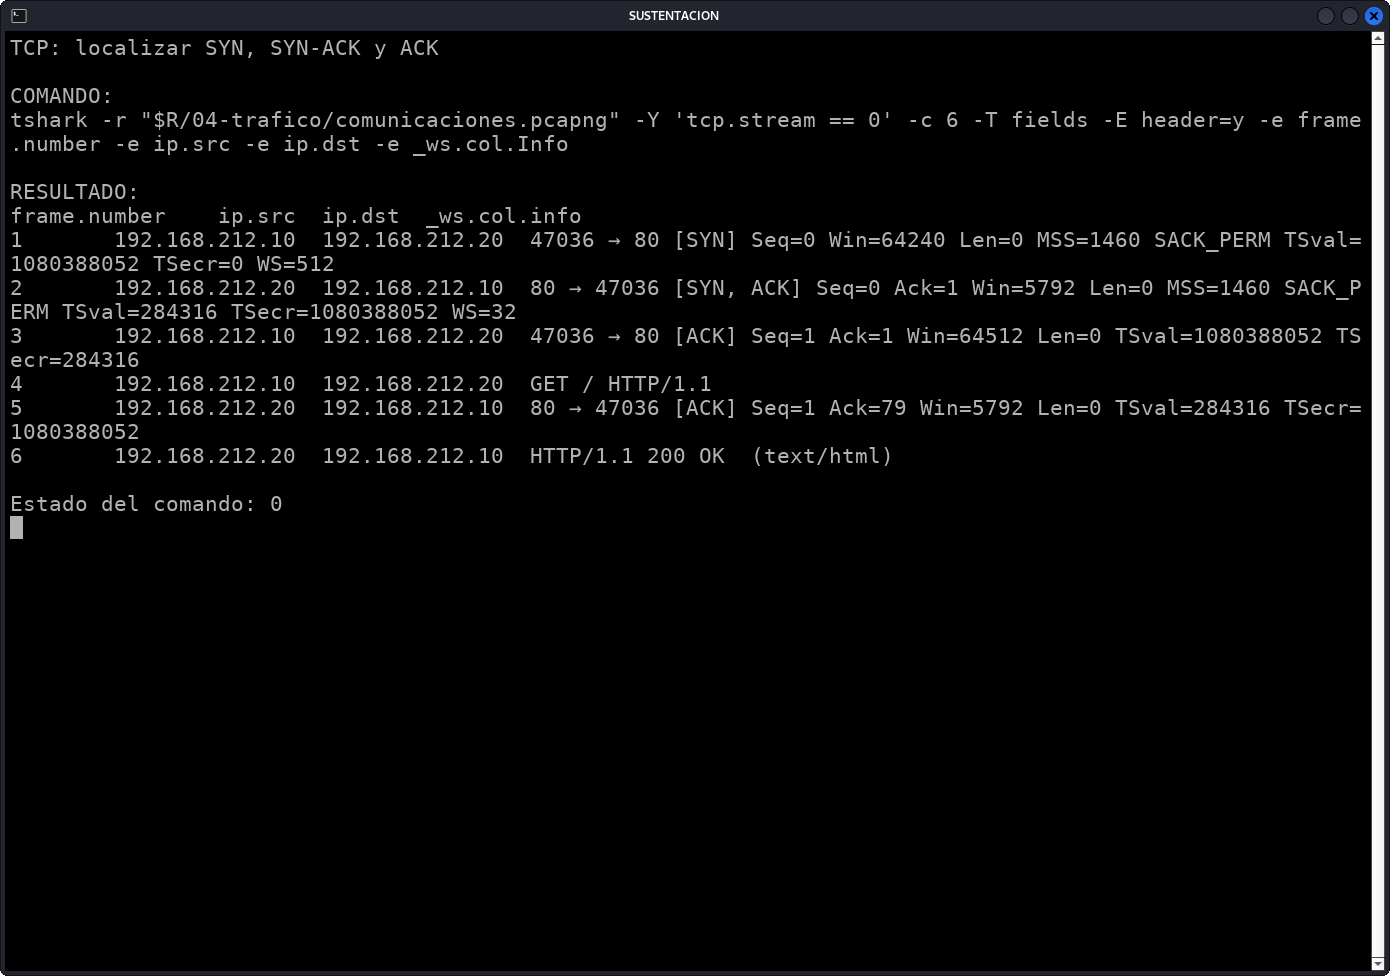
\includegraphics[width=1.0\linewidth,trim=0 414bp 0 0,clip]{sustentacion/08-tcp.png}\caption{Consulta de la conversación TCP desde la terminal.}\end{figure}

\begin{figure}[H]\centering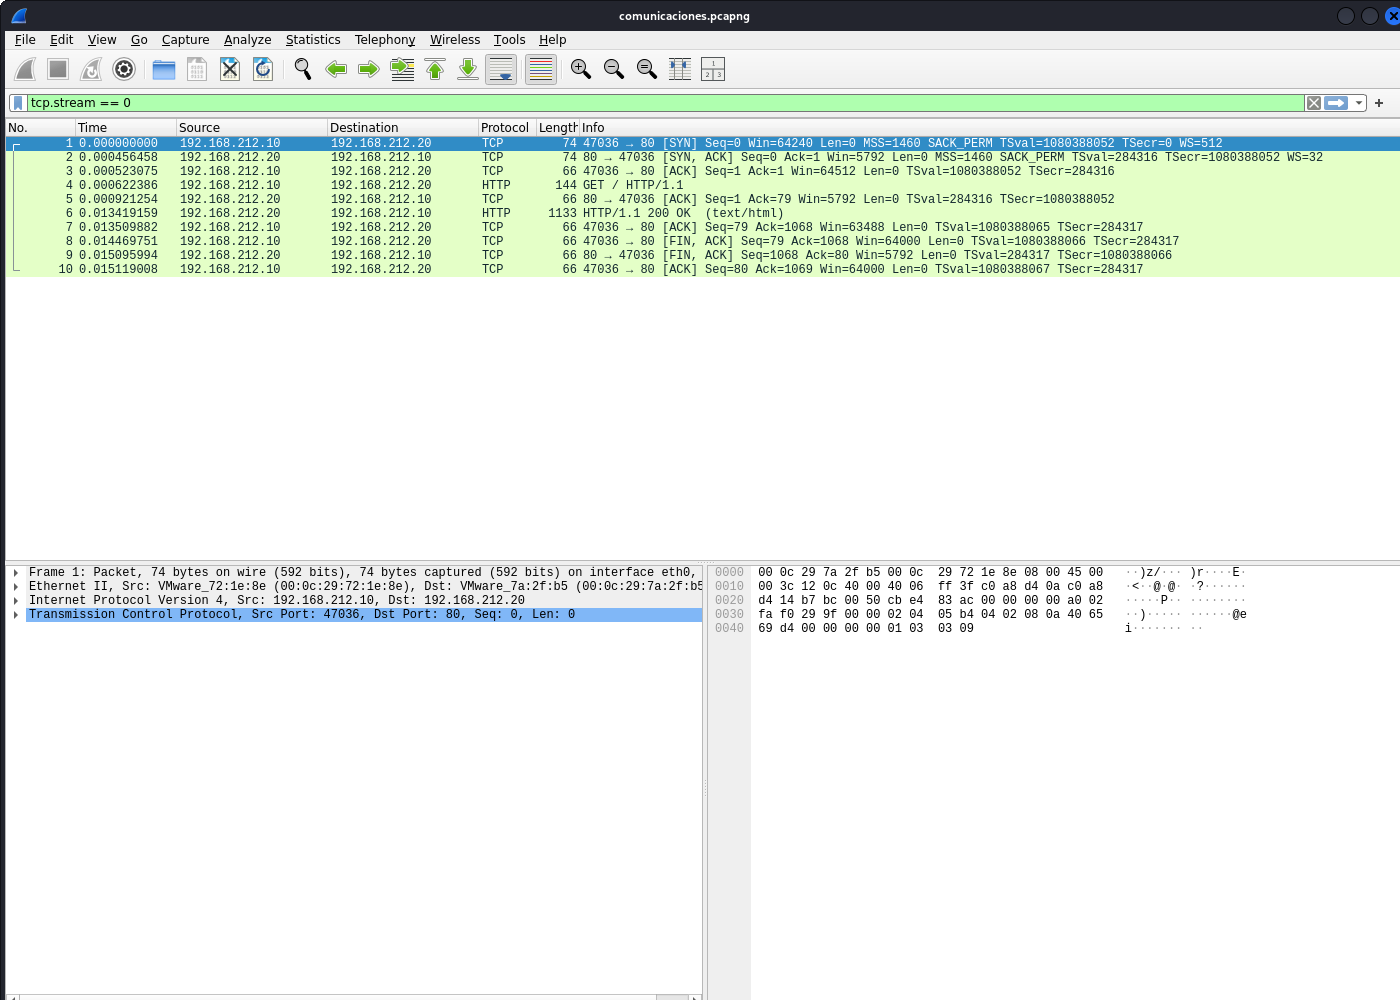
\includegraphics[width=1.0\linewidth,trim=0 0bp 0 0,clip]{sustentacion/16-wireshark-tcp.png}\caption{La misma conversación abierta en Wireshark.}\end{figure}

\par\textbf{Lectura.} Source y Destination indican origen y destino. La columna Info permite reconocer los indicadores TCP. Un stream es una conversación; el filtro \texttt{tcp.stream == 0} selecciona esta conexión en la corrida actual. El número puede cambiar en otra captura.
\clearpage\section*{4. Tráfico: relacionar la solicitud y respuesta HTTP}\label{http}

\begin{figure}[H]\centering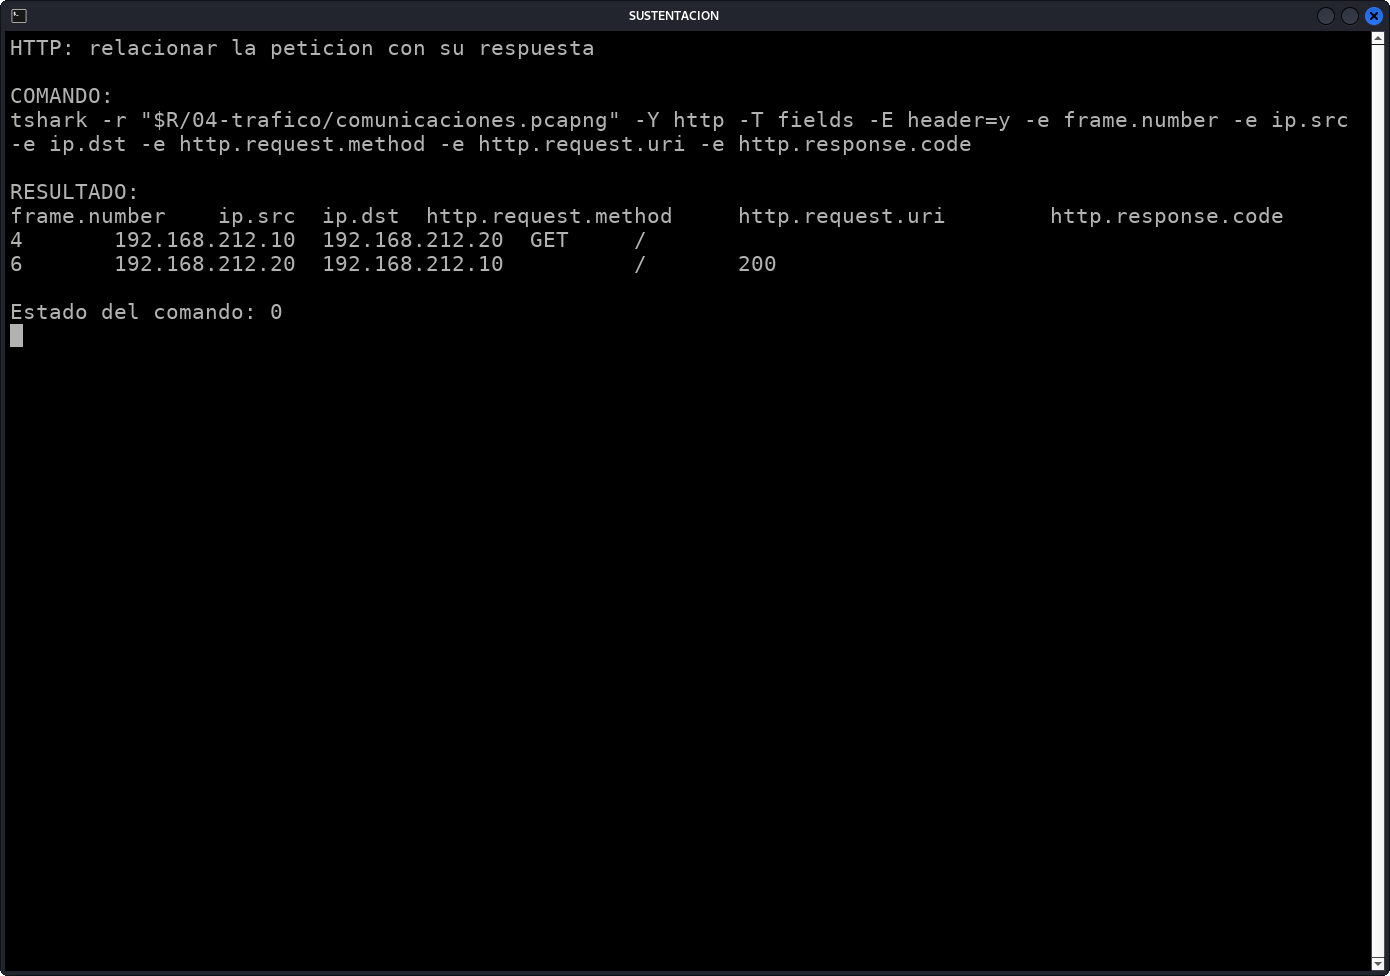
\includegraphics[width=1.0\linewidth,trim=0 606bp 0 0,clip]{sustentacion/09-http-analisis.png}\caption{TShark extrae las filas HTTP, direcciones y resultado de la consulta.}\end{figure}

\begin{figure}[H]\centering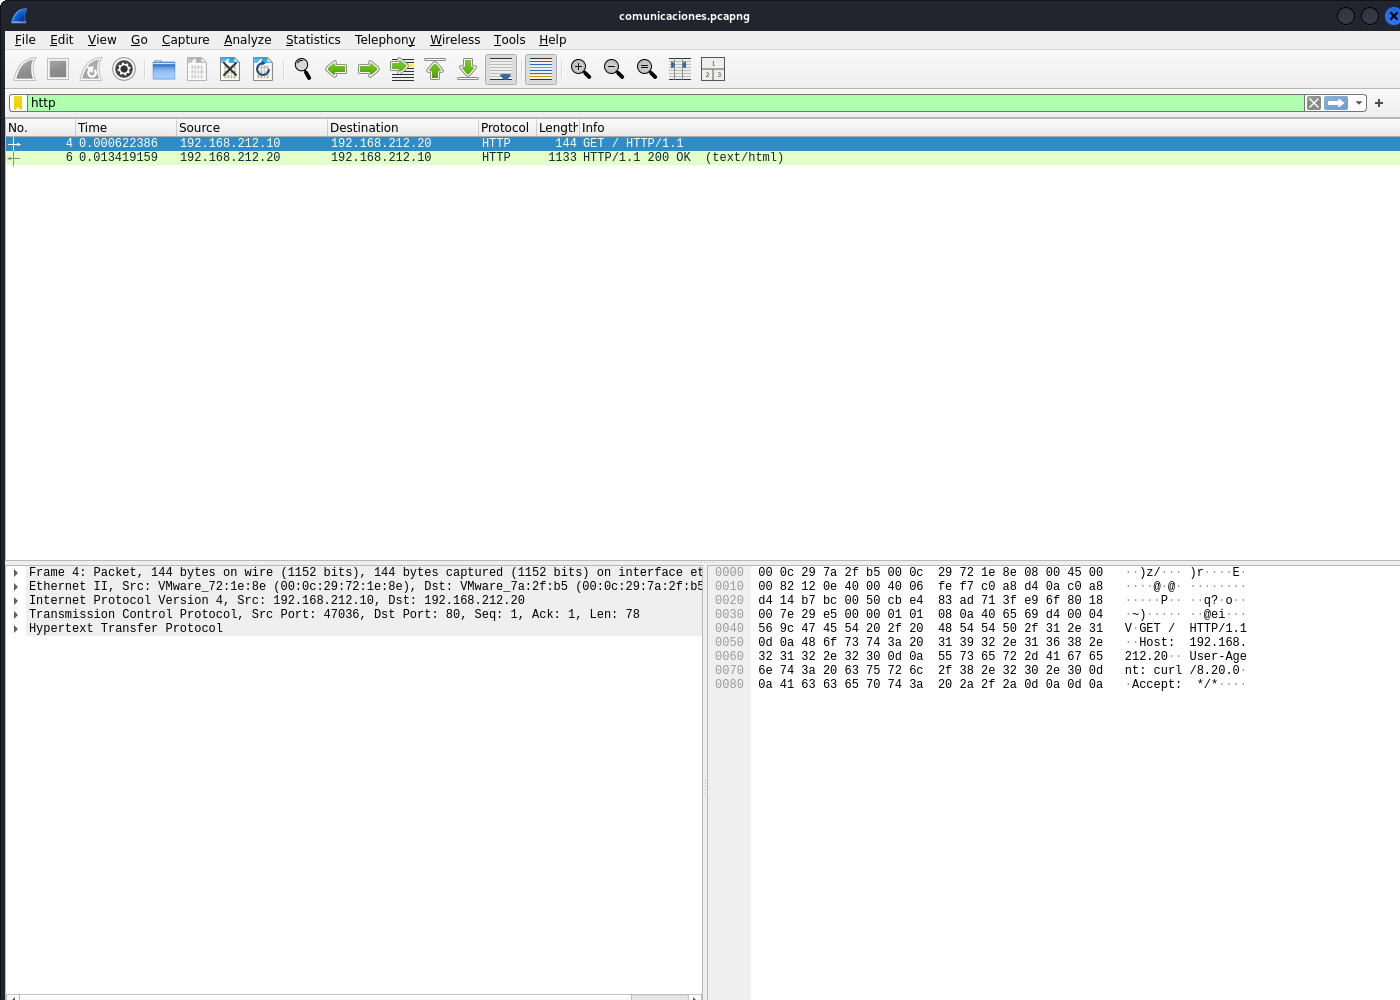
\includegraphics[width=1.0\linewidth,trim=0 0bp 0 0,clip]{sustentacion/17-wireshark-http.png}\caption{Filtro HTTP en Wireshark sobre el mismo archivo de tráfico.}\end{figure}

\par\textbf{Lectura.} Las filas HTTP son 4, 6. La petición \texttt{GET /} va de Kali hacia \texttt{.20:80}; la respuesta \texttt{200} vuelve desde la víctima. Al seleccionar una fila, el panel intermedio presenta los protocolos y el inferior sus bytes. Se puede interpretar el contenido sin descifrarlo: esta sesión no utilizó TLS (Transport Layer Security, protección criptográfica del canal).
\clearpage\section*{4. Tráfico: reconocer las consultas y respuestas Modbus}\label{modbus}

\begin{figure}[H]\centering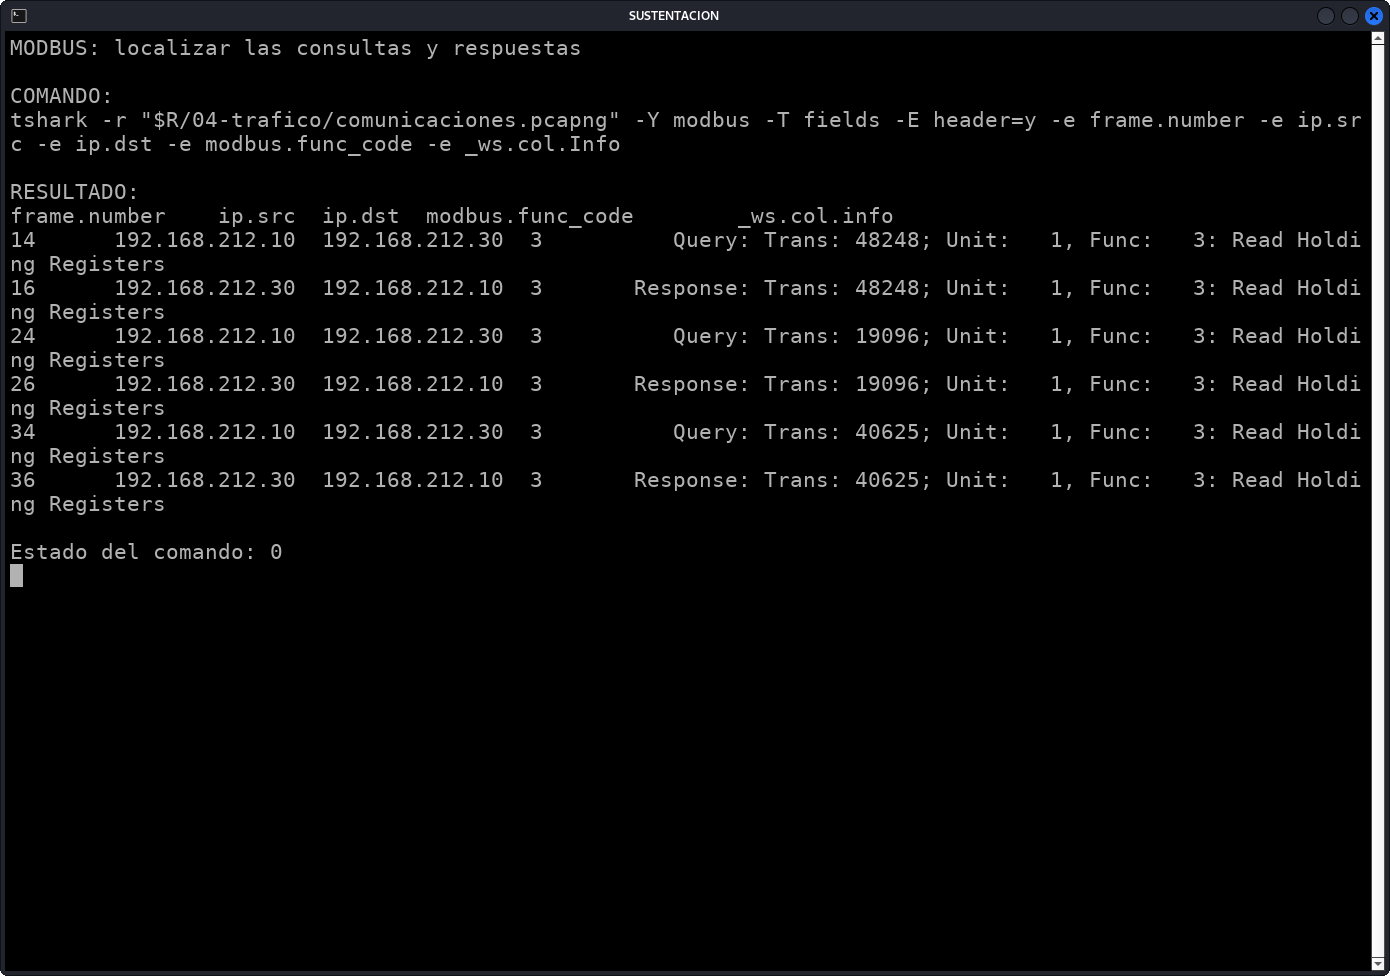
\includegraphics[width=1.0\linewidth,trim=0 366bp 0 0,clip]{sustentacion/10-modbus-analisis.png}\caption{Extracción de las tramas Modbus mediante TShark.}\end{figure}

\begin{figure}[H]\centering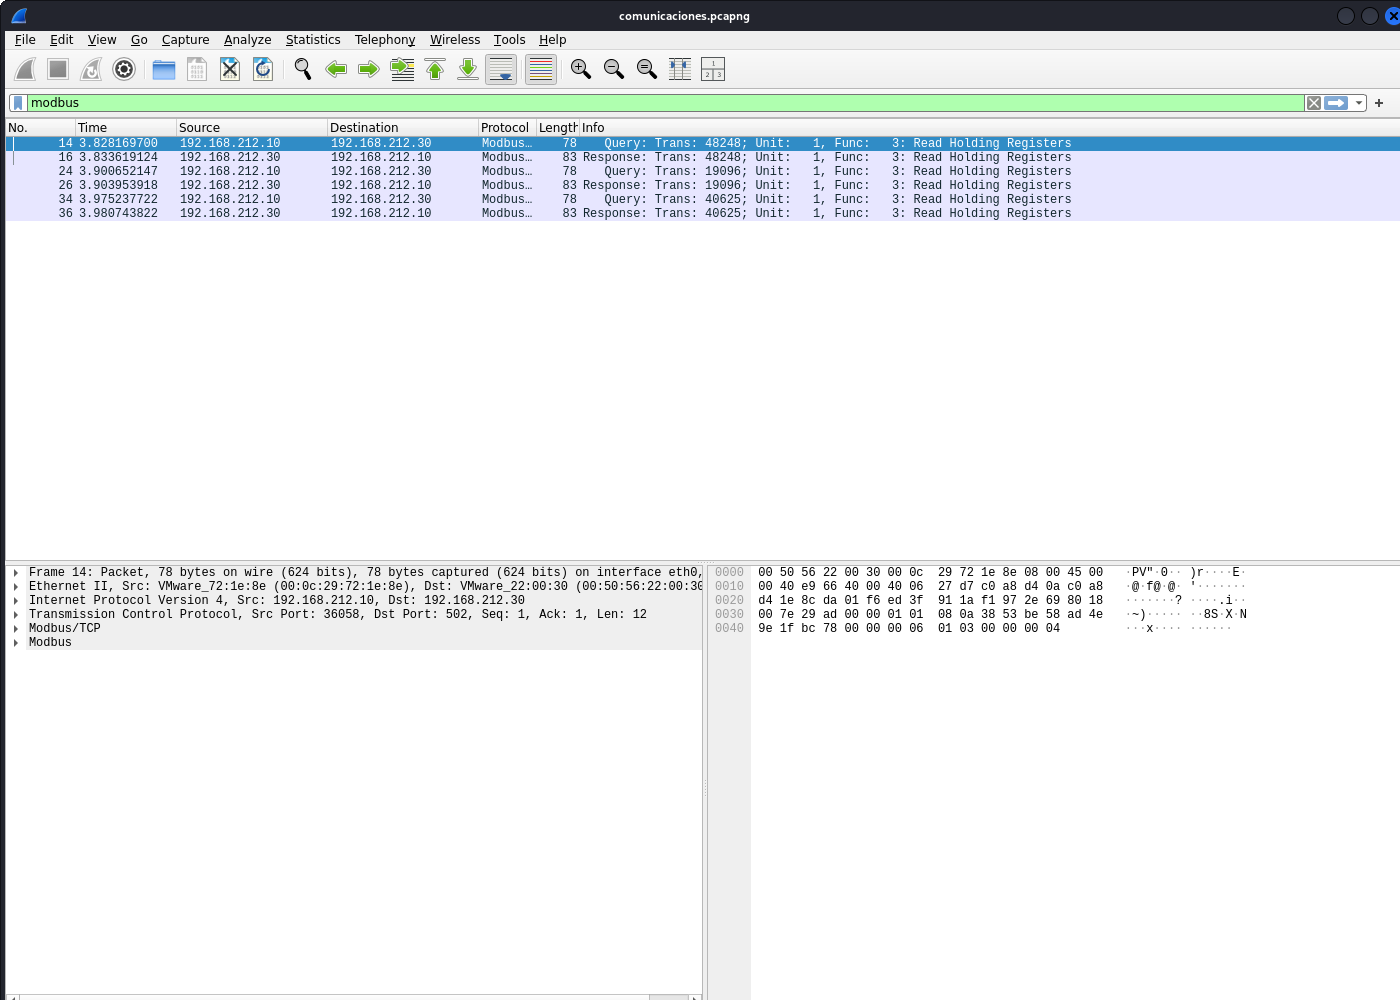
\includegraphics[width=1.0\linewidth,trim=0 0bp 0 0,clip]{sustentacion/18-wireshark-modbus.png}\caption{Filtro Modbus y las respuestas del PLC simulado.}\end{figure}

\par\textbf{Lectura.} Las filas identificadas son 14, 16, 24, 26, 34, 36. Las peticiones van de \texttt{.10} a \texttt{.30:502}; las respuestas regresan con los registros. El filtro \texttt{modbus} selecciona el protocolo y \texttt{tcp.port == 502} selecciona ese puerto. Los números de trama identifican filas de este archivo; no son pasos del procedimiento. Las lecturas sin autenticación y el contenido legible justifican restringir qué clientes acceden al PLC.
\clearpage\section*{5. Identificación de riesgos de seguridad}\label{riesgos}

Se relacionó cada condición con una observación concreta. El impacto describe lo que podría ocurrir; se mantiene separado de las acciones efectivamente realizadas.
\par\begin{tabularx}{\linewidth}{@{}P{3.6cm}YY@{}}\toprule
Condición & Evidencia & Impacto potencial\\\midrule
Credencial predeterminada & Telnet aceptó \texttt{msfadmin/msfadmin}. & Asumir esa identidad con un secreto público.\\
Telnet sin cifrado & Usuario y contraseña se recuperan de la captura de red. & Exposición a quien pueda observar el trayecto o acceder a la captura.\\
HTTP sin protección del canal & Solicitud y respuesta legibles. & Exposición del contenido si se transmitieran datos sensibles. Aquí se leyó una página pública.\\
Lectura Modbus sin autenticación & Un cliente de la red obtuvo cuatro registros. & Consulta no autorizada de información industrial; no se probó escritura ni un proceso físico.\\\bottomrule
\end{tabularx}
\textbf{Cómo se investigó.} Rapid7 es la empresa cuya documentación describe Metasploitable y su credencial pública [1]. MITRE es una organización que participa en iniciativas de conocimiento de ciberseguridad [4]. Se consultó el catálogo CWE (Common Weakness Enumeration), que clasifica tipos de debilidades: CWE-1392 corresponde al uso de credenciales predeterminadas; CWE-319, a información sensible transmitida en claro [2--3]. Son fuentes y categorías, no aplicaciones ejecutadas contra la víctima.
\textbf{CWE y CVE.} CVE significa Common Vulnerabilities and Exposures y da identificadores a vulnerabilidades concretas divulgadas públicamente [5]. Aquí se comprobaron condiciones de configuración y comunicación inseguras; no se demostró explotación de una CVE específica.

\clearpage\section*{6. Evidencia de una prueba controlada de vulnerabilidad}\label{telnet-inicio}

\par\textbf{1. Abrir Telnet en la víctima.} Telnet permite interactuar con la terminal de otro equipo. El cliente de Kali se conecta al servidor \texttt{.20:23}; TCP transporta sus bytes sin cifrarlos por sí mismo [6]. La prueba empleó únicamente la credencial pública de la máquina didáctica.
\begin{figure}[H]\centering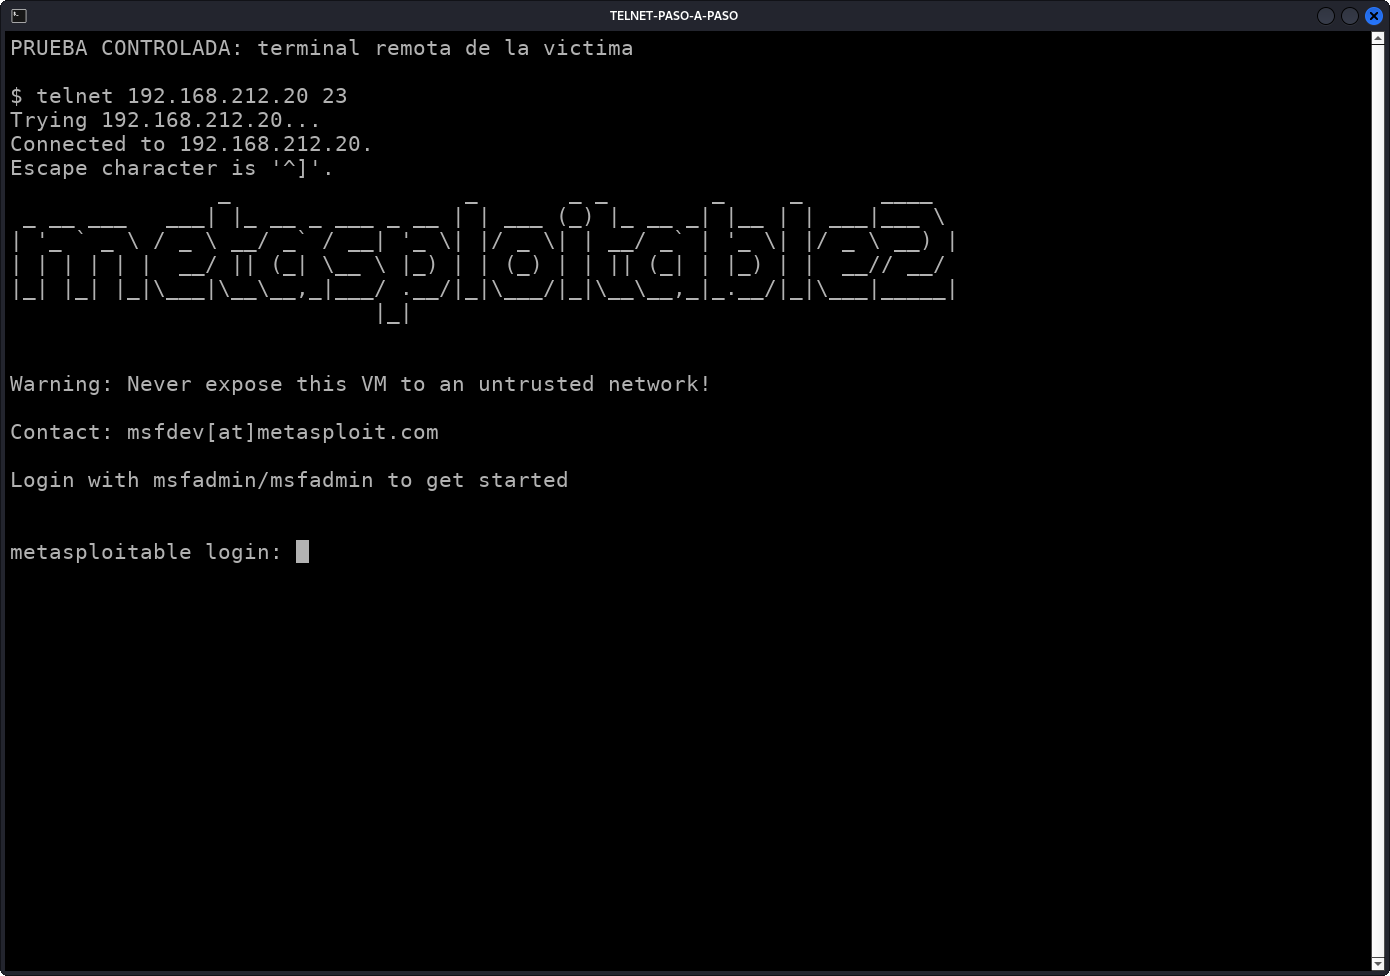
\includegraphics[width=1.0\linewidth,trim=0 390bp 0 0,clip]{sustentacion/11a-telnet-login.png}\caption{Conexión al puerto 23 y solicitud de usuario.}\end{figure}

\par\textbf{2. Introducir el usuario.} Se escribió \texttt{msfadmin}; el servidor pidió la contraseña. Que la terminal no muestre caracteres al escribirla solo evita el eco en pantalla, no demuestra cifrado de la red.
\begin{figure}[H]\centering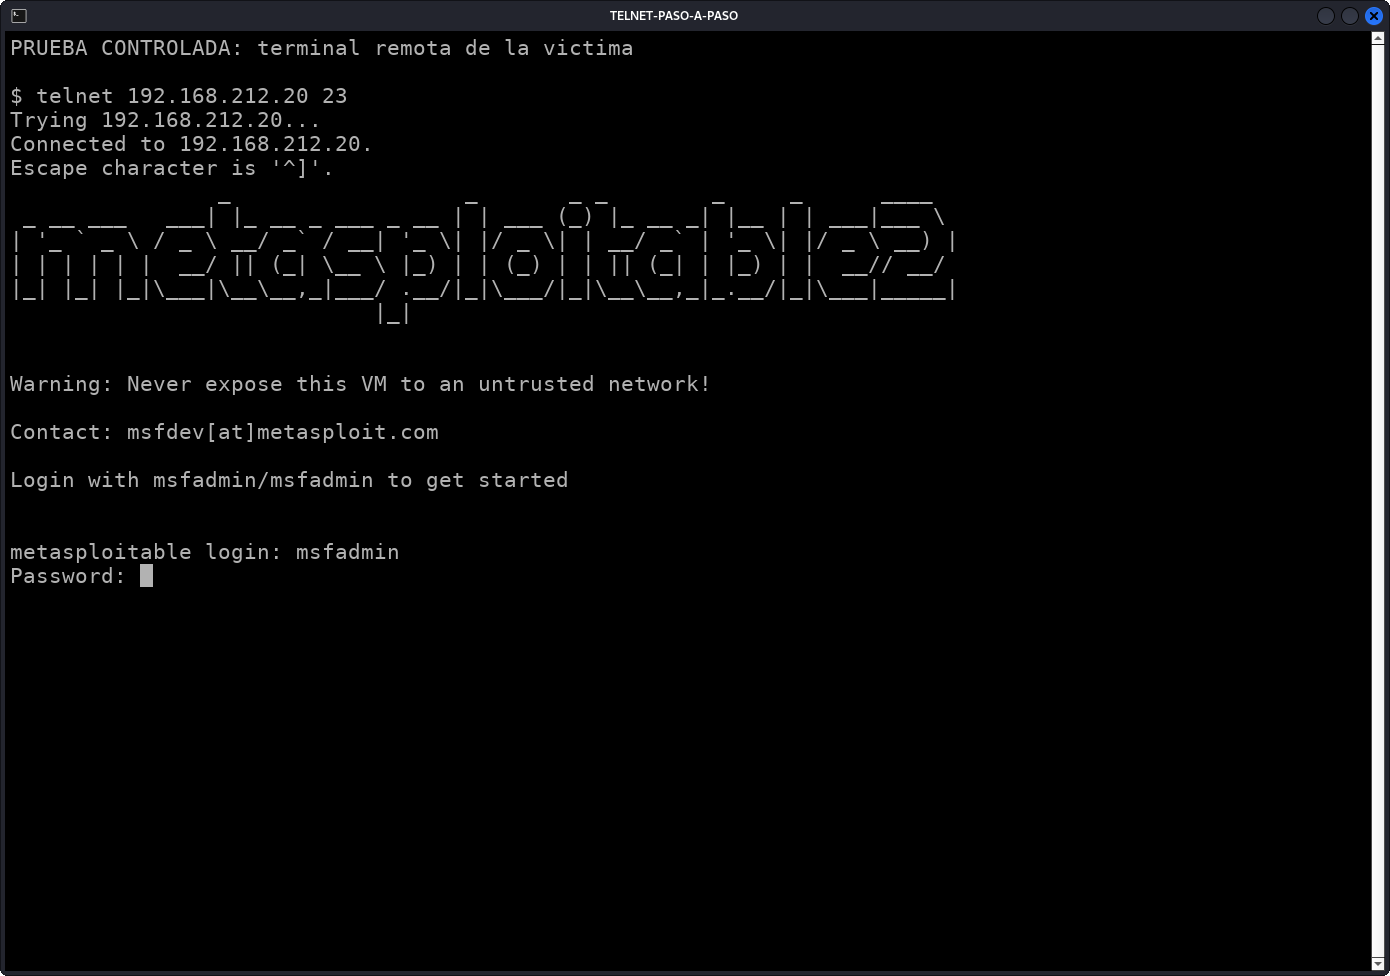
\includegraphics[width=1.0\linewidth,trim=0 366bp 0 0,clip]{sustentacion/11b-telnet-password.png}\caption{El servidor solicita la contraseña después del usuario.}\end{figure}

\clearpage\section*{6. Prueba controlada: comprobar identidad y cerrar}\label{telnet-comandos}

\par\textbf{3. Comprobar la identidad.} Tras aceptar \texttt{msfadmin} como contraseña se consultó \texttt{id}. Se limpió la pantalla para que se pudiera leer el resultado; limpiar la terminal no elimina los mensajes ya capturados en la red.
\begin{quote}\ttfamily\small\raggedright id\par\end{quote}

\begin{figure}[H]\centering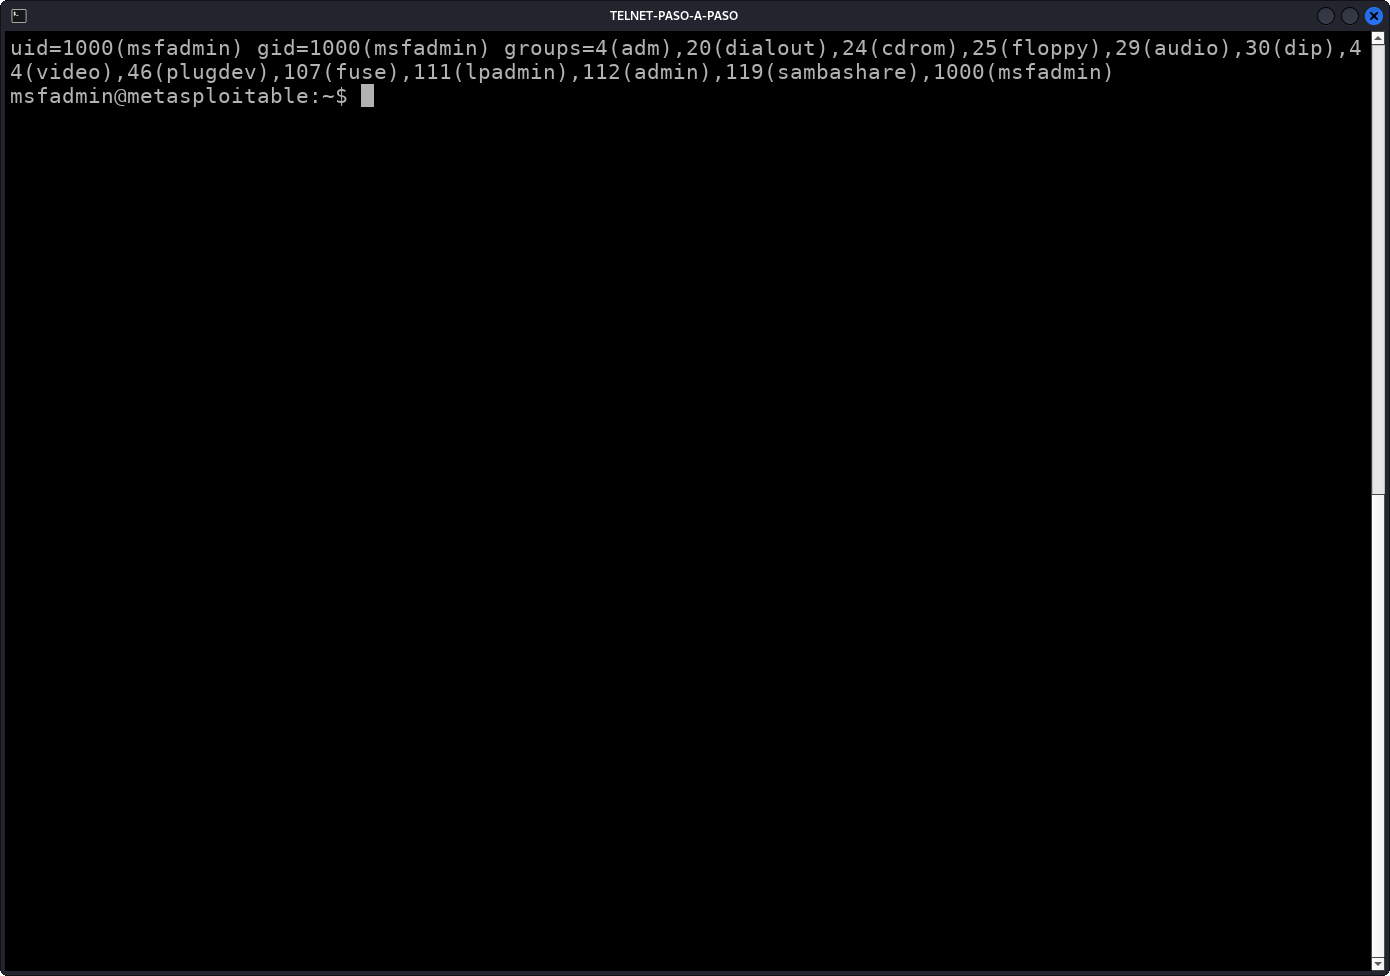
\includegraphics[width=1.0\linewidth,trim=0 846bp 0 0,clip]{sustentacion/11c-telnet-identidad.png}\caption{La terminal de la víctima muestra la identidad msfadmin.}\end{figure}

\par\textbf{Lectura.} \texttt{uid=1000(msfadmin)} identifica al usuario de la sesión; UID es el identificador de usuario. Root es la cuenta administrativa de UID 0, por lo que este resultado no acredita acceso root.
\par\textbf{4. Consultar el sistema y salir.} \texttt{uname -a} informa el sistema y su núcleo; \texttt{exit} cierra la conexión. Estas órdenes no solicitan modificar archivos ni elevar privilegios.
\begin{figure}[H]\centering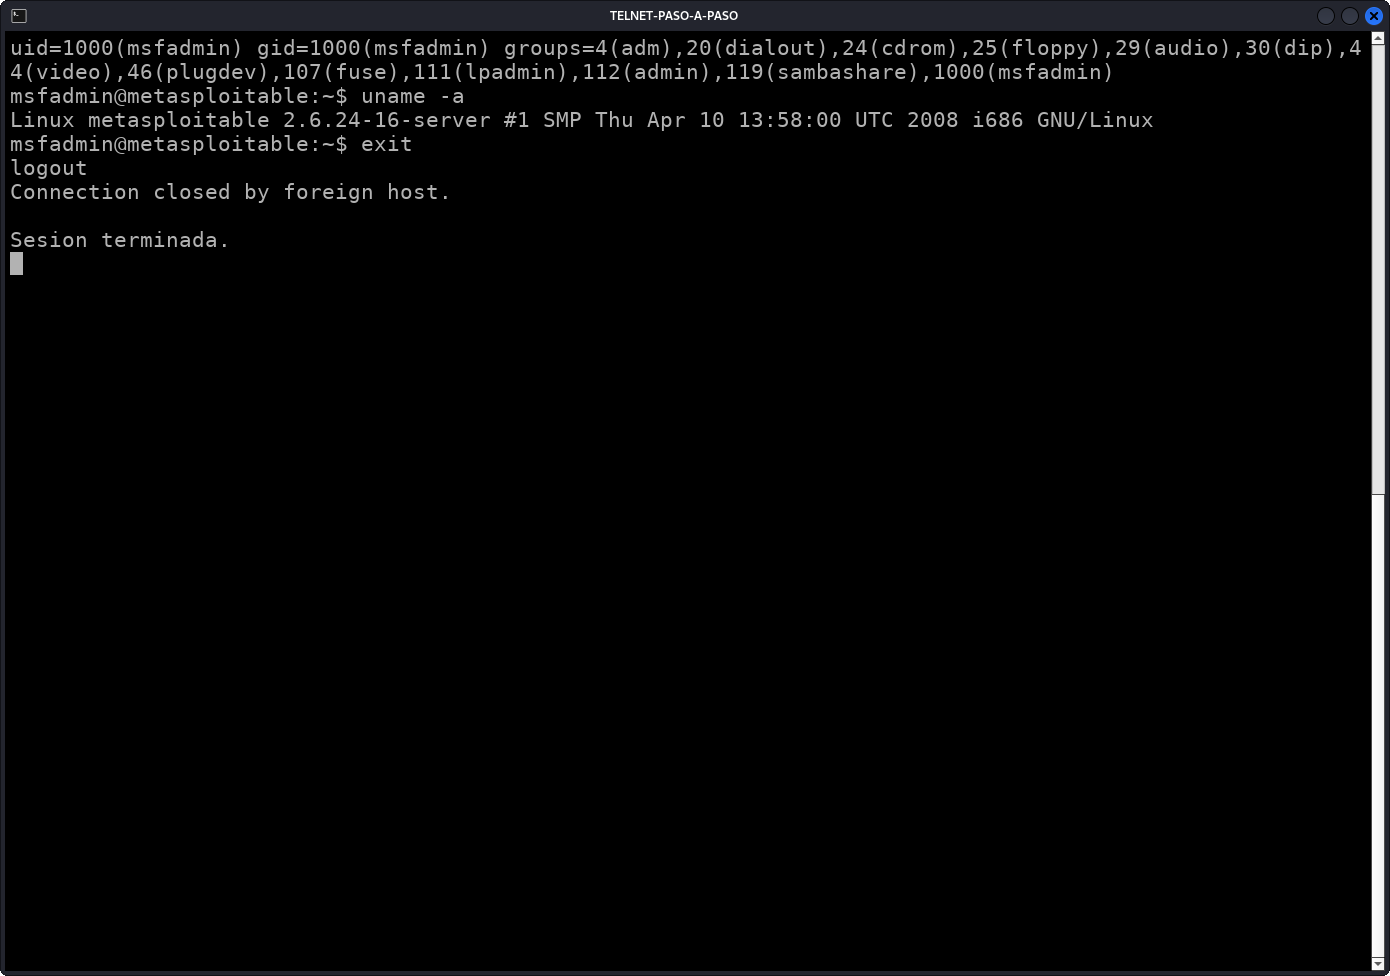
\includegraphics[width=1.0\linewidth,trim=0 678bp 0 0,clip]{sustentacion/11d-telnet-cierre.png}\caption{Consulta del sistema y cierre de la sesión remota.}\end{figure}

\clearpage\section*{6. Prueba controlada: contrastar la sesión con la red}\label{telnet-trafico}

\par\textbf{5. Leer la captura específica de Telnet.} Se registró esta sesión en \texttt{06-prueba/telnet.pcapng}, separada de HTTP/Modbus. La transcripción de la terminal muestra el acceso aceptado; el PCAP permite revisar los bytes enviados durante la misma sesión.
\begin{figure}[H]\centering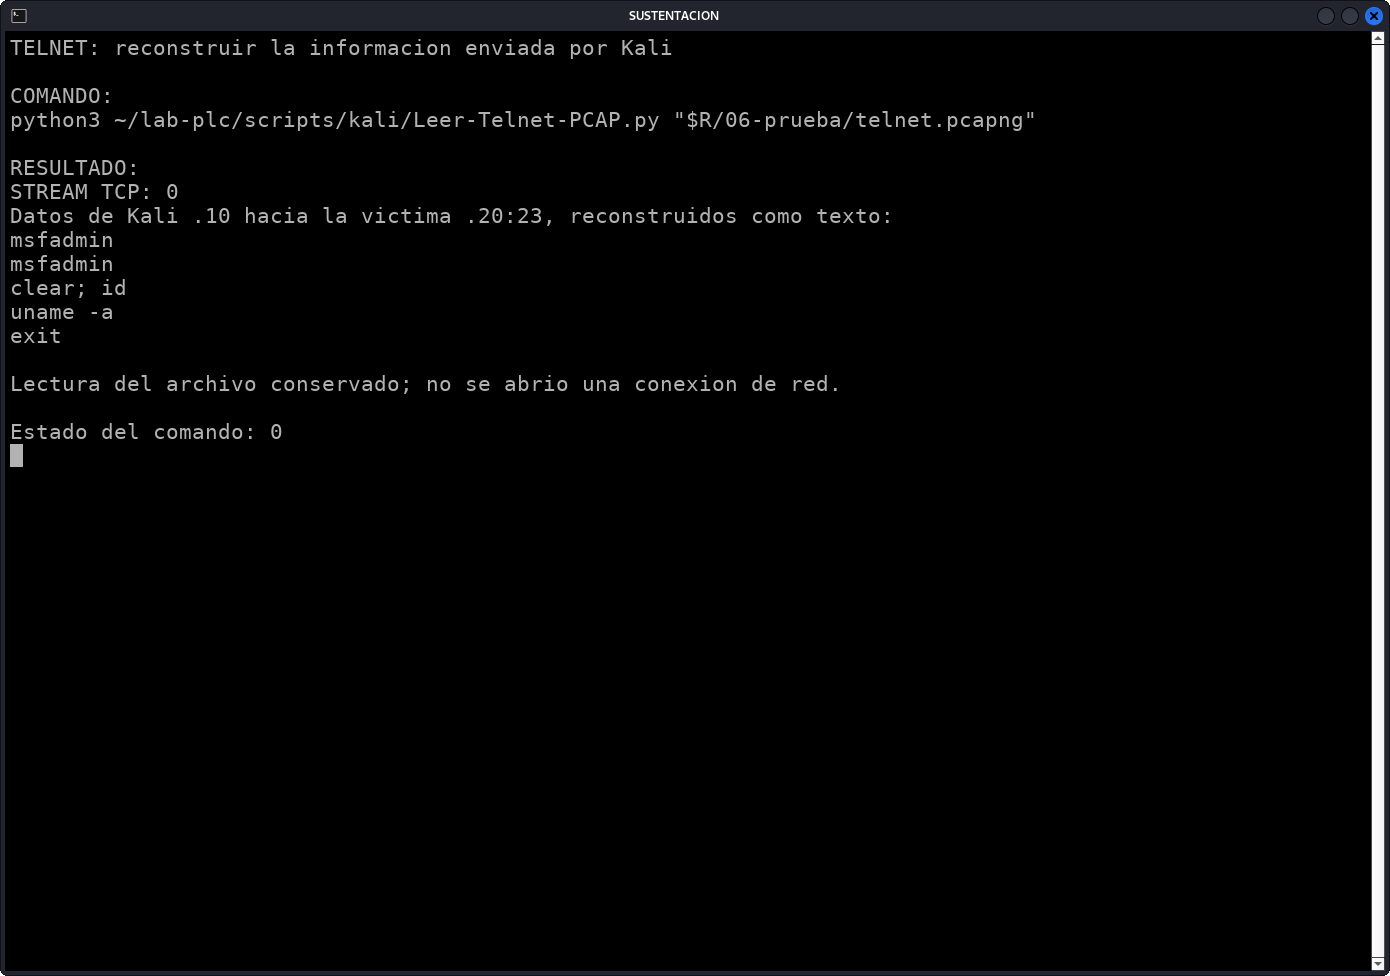
\includegraphics[width=1.0\linewidth,trim=0 486bp 0 0,clip]{sustentacion/12-telnet-trafico.png}\caption{Reconstrucción como texto de los datos que Kali envió durante la sesión.}\end{figure}

\begin{figure}[H]\centering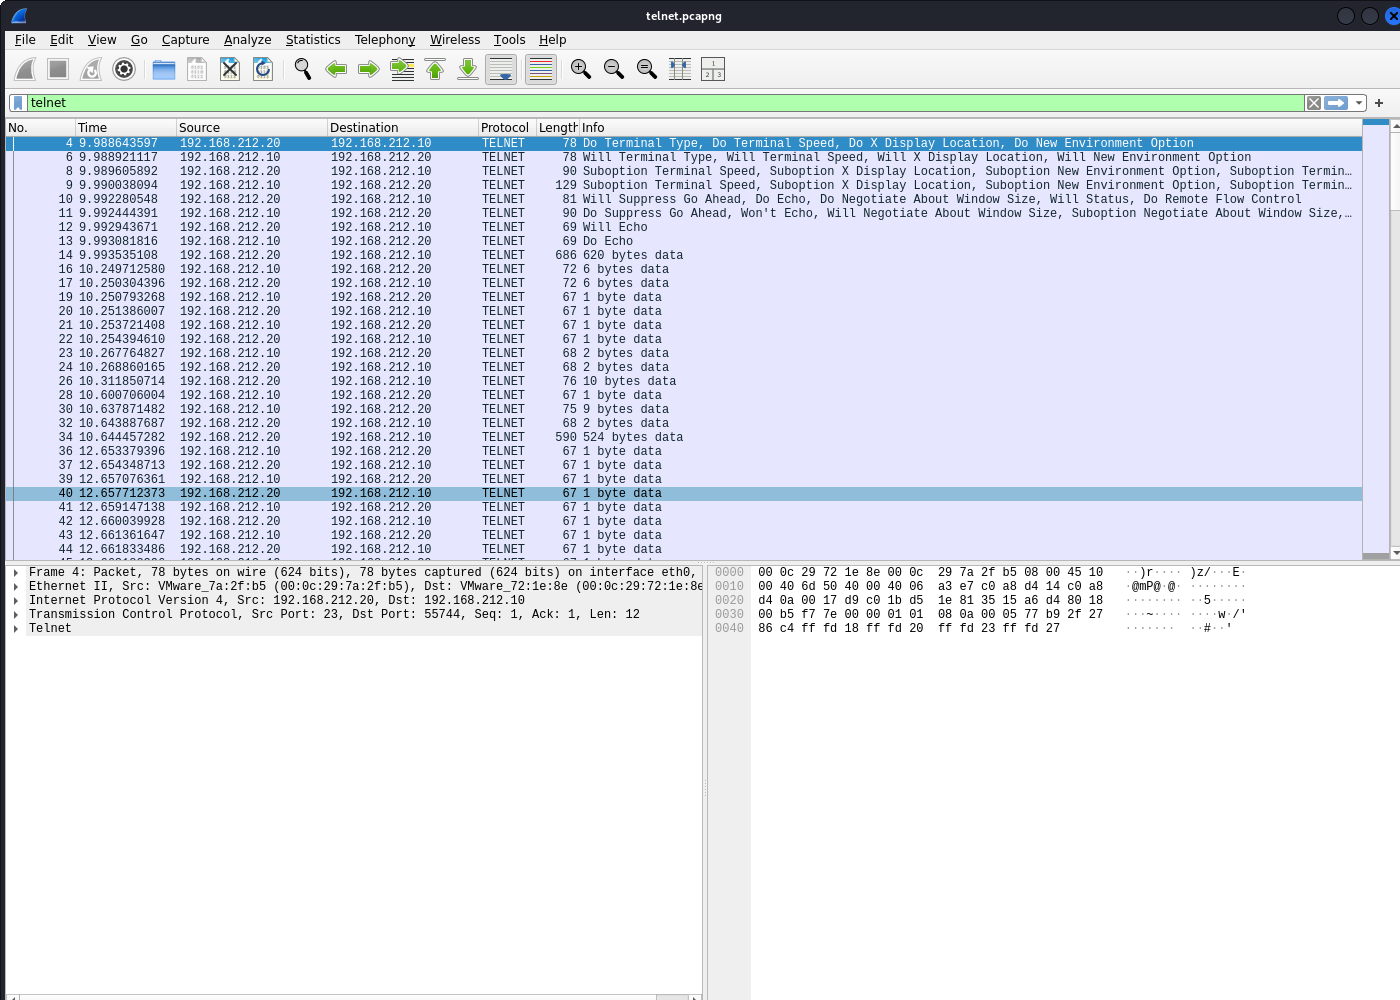
\includegraphics[width=1.0\linewidth,trim=0 0bp 0 0,clip]{sustentacion/19-wireshark-telnet.png}\caption{Sesión Telnet vista en Wireshark.}\end{figure}

\par\textbf{Lectura.} La primera vista reconstruye los datos TCP del cliente con TShark y elimina los controles propios de Telnet para mostrar el texto: aparecen el usuario, la contraseña y las órdenes. En Wireshark se puede seleccionar una fila y usar \emph{Follow / TCP Stream}, mostrando texto ASCII. ``En claro significa que ese contenido se interpreta sin una clave de descifrado. La contraseña puede repartirse en varias tramas: por eso se revisa la conversación completa, no un número fijo. No se afirma que un tercero haya interceptado esta sesión.
\clearpage\section*{7. Cálculo y verificación de hashes SHA-256}\label{hash1}

\par\textbf{1. Seleccionar y conservar.} Se eligió el PCAP HTTP/Modbus de esta demostración y se creó \texttt{original.evidencia} sin permiso de escritura. SHA-256 (Secure Hash Algorithm de 256 bits) produce un resumen de los bytes; permite compararlos con una referencia, sin cifrar el archivo.
\begin{figure}[H]\centering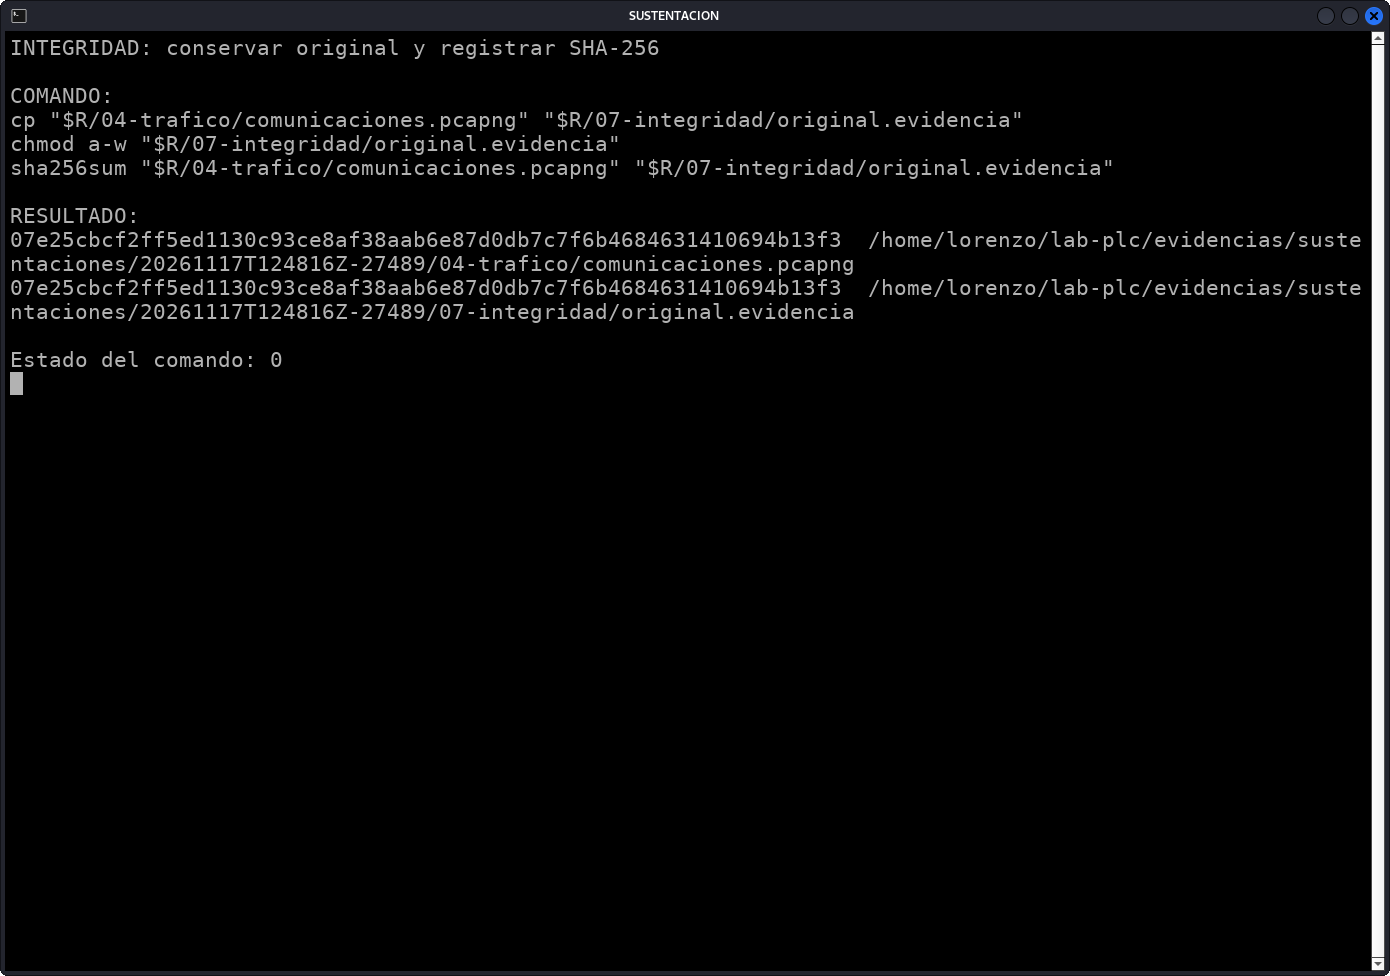
\includegraphics[width=1.0\linewidth,trim=0 558bp 0 0,clip]{sustentacion/13-hash-original.png}\caption{La fuente y su copia original producen el mismo SHA-256.}\end{figure}

\par\textbf{2. Cambiar solo otra copia.} Se creó \texttt{copia-alterada.evidencia} y se añadió una línea de prueba. La fuente quedó conservada; el cambio fue de 39 bytes.
\begin{figure}[H]\centering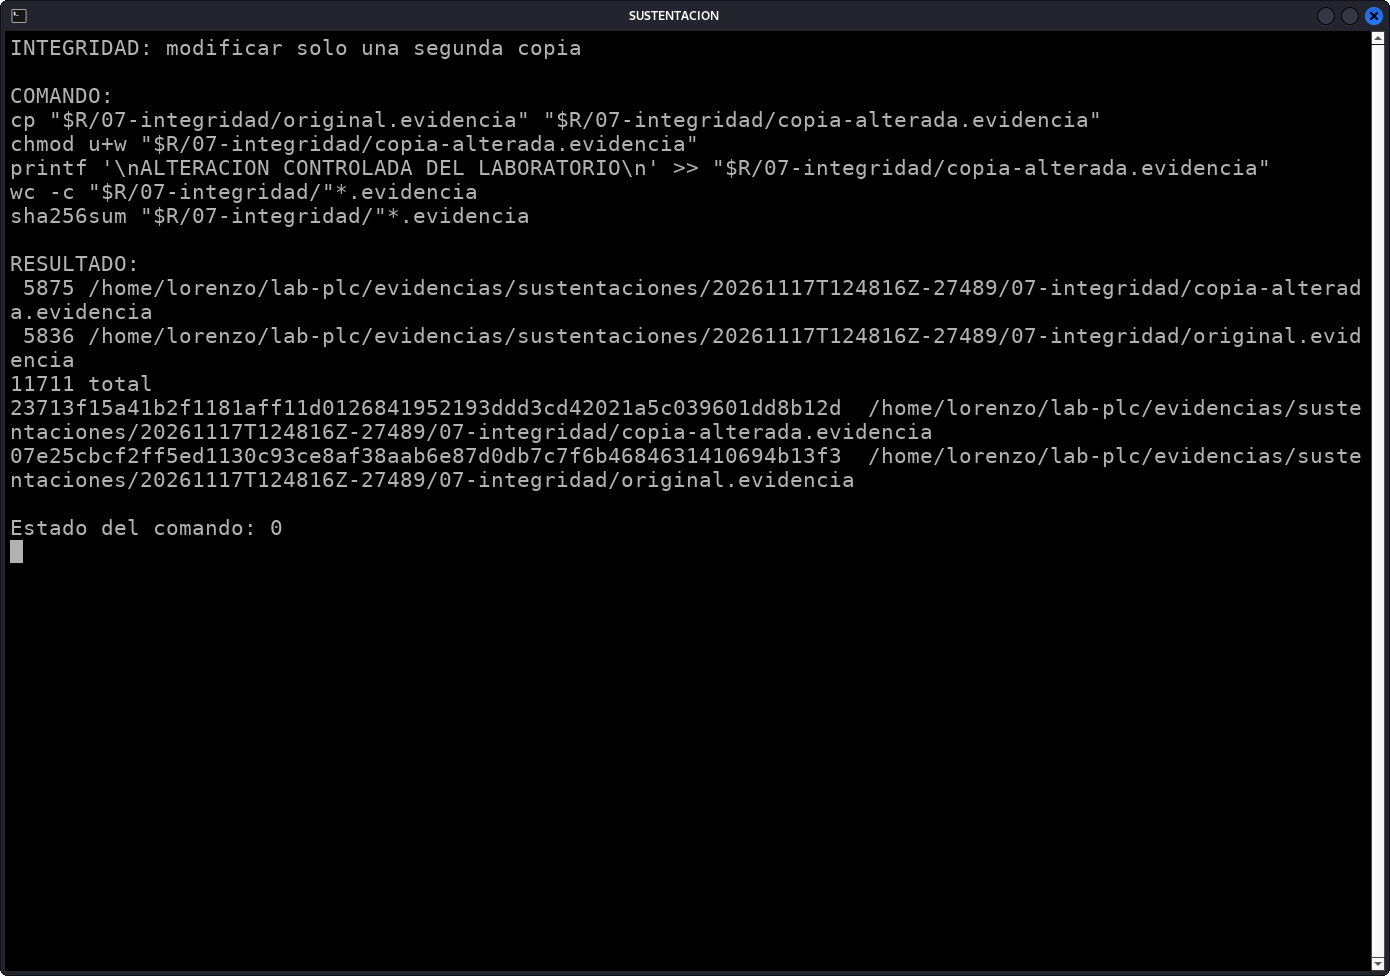
\includegraphics[width=1.0\linewidth,trim=0 390bp 0 0,clip]{sustentacion/14-copia-alterada.png}\caption{Tamaño y hash después de modificar únicamente la segunda copia.}\end{figure}

\clearpage\section*{7. Integridad: registrar, verificar y comparar}\label{hash2}

\begin{figure}[H]\centering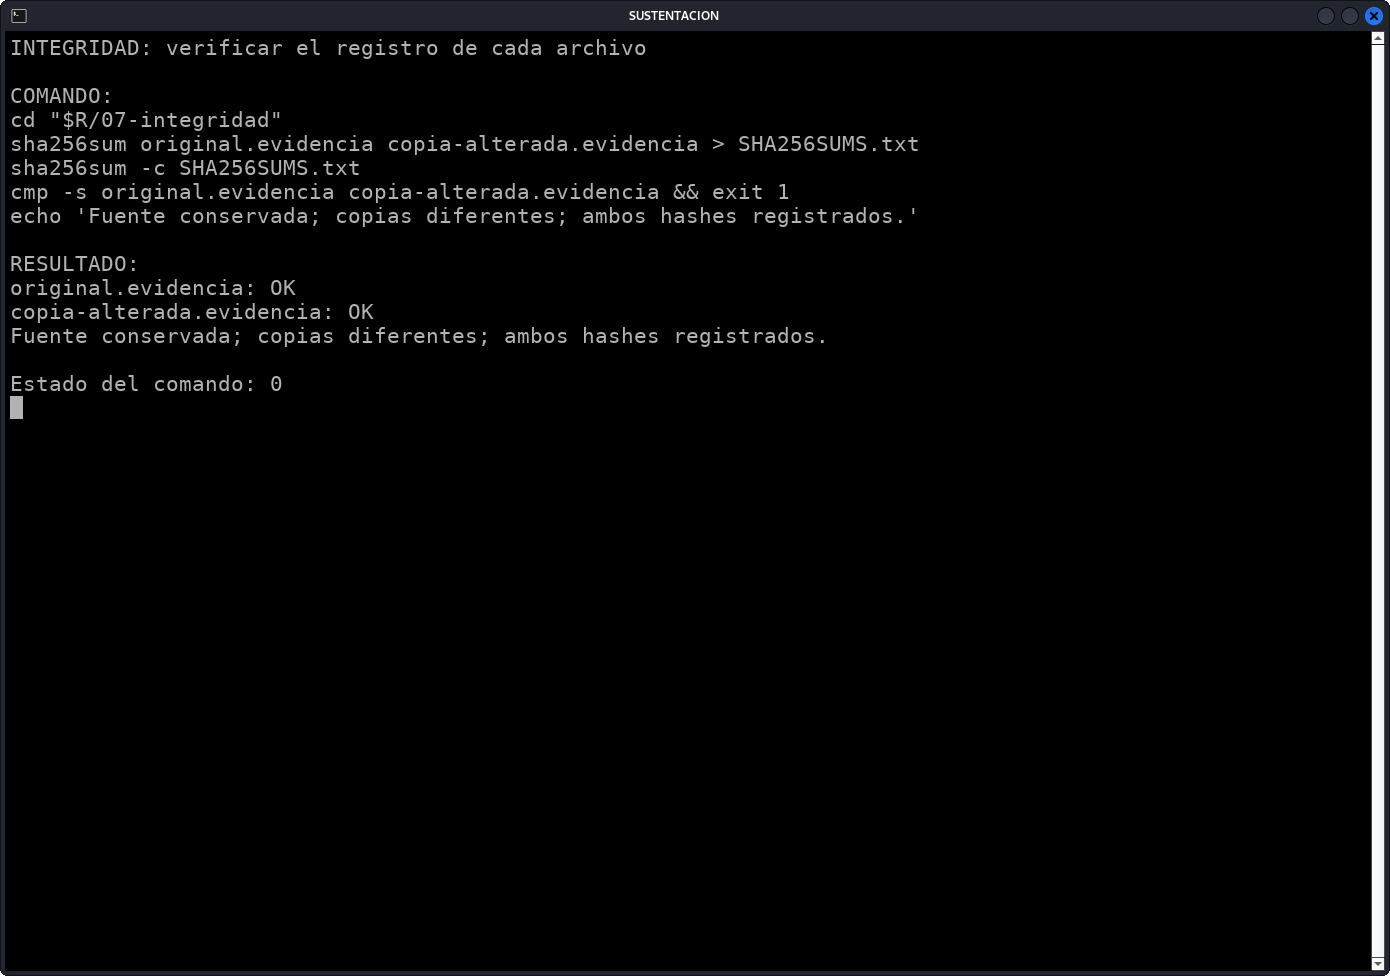
\includegraphics[width=1.0\linewidth,trim=0 534bp 0 0,clip]{sustentacion/15-verificacion.png}\caption{Registro y comprobación de los hashes de ambas copias.}\end{figure}

\par\textbf{3. Interpretar el resultado.} Cada \texttt{OK} significa que el archivo coincide con su propia entrada en \texttt{SHA256SUMS.txt}; no que ambas copias sean iguales. La comparación detectó diferencia entre el original y la copia alterada. Un hash aislado no demuestra autoría ni una cadena de custodia completa.
\par\begin{tabularx}{\linewidth}{@{}P{3cm}Y@{}}\toprule Archivo & SHA-256 completo\\\midrule
Fuente / original & {\ttfamily\small 07e25cbcf2ff5ed1130c93ce8af38aab\newline 6e87d0db7c7f6b4684631410694b13f3}\\[5pt]
Copia alterada & {\ttfamily\small 23713f15a41b2f1181aff11d01268419\newline 52193ddd3cd42021a5c039601dd8b12d}\\[5pt]
\bottomrule\end{tabularx}
\par\textbf{Tamaños.} El original tiene 5836 bytes y la copia alterada 5875. El manifiesto completo de la corrida y las imágenes se conservan junto a los resultados originales de los comandos.
\clearpage\section*{7. Integridad: inspección complementaria de archivos}\label{ftk}

FTK Imager es una herramienta para incorporar e inspeccionar evidencias digitales. Se conserva también la revisión de la carpeta de tráfico original del 12 de noviembre: en esa corrida el PCAP tenía 20.940 bytes. Estas dos imágenes corresponden a esa revisión anterior, separada de los hashes de la nueva demostración.
\textbf{1. Incorporar la carpeta.} File / Add Evidence Item / Contents of a Folder añadió \texttt{02-trafico}. Evidence Tree muestra la fuente incorporada.
\begin{figure}[H]\centering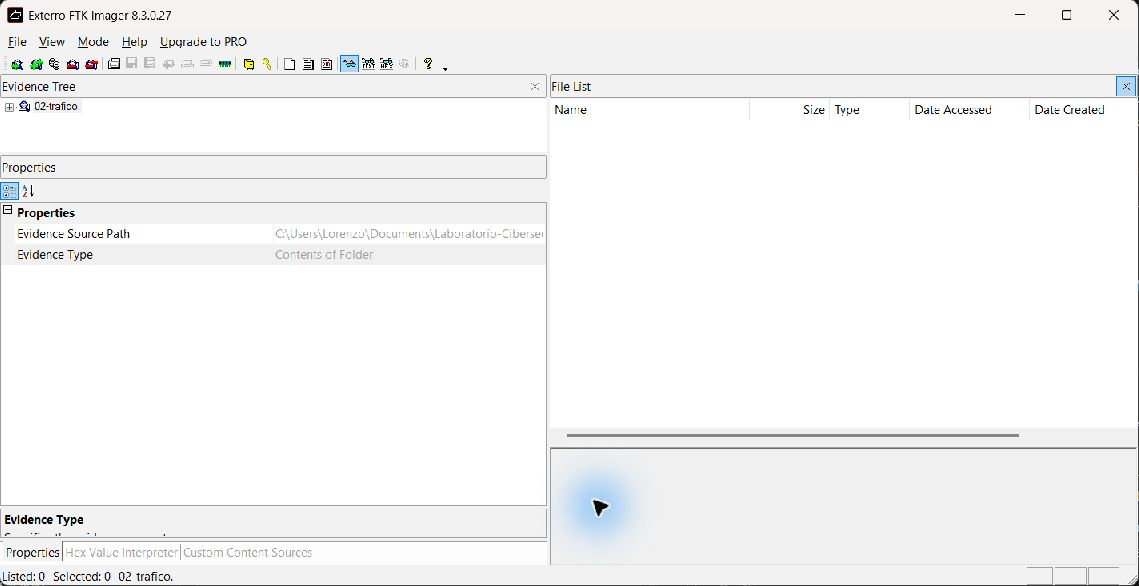
\includegraphics[width=0.78\linewidth]{06-ftk-carpeta.jpg}\caption{Carpeta original incorporada como fuente en FTK Imager.}\end{figure}
\textbf{2. Seleccionar el archivo.} Al desplegar la carpeta se seleccionó \texttt{comunicaciones.pcapng}. Las propiedades muestran nombre, tamaño y tipo; el panel inferior presenta sus bytes en hexadecimal.
\begin{figure}[H]\centering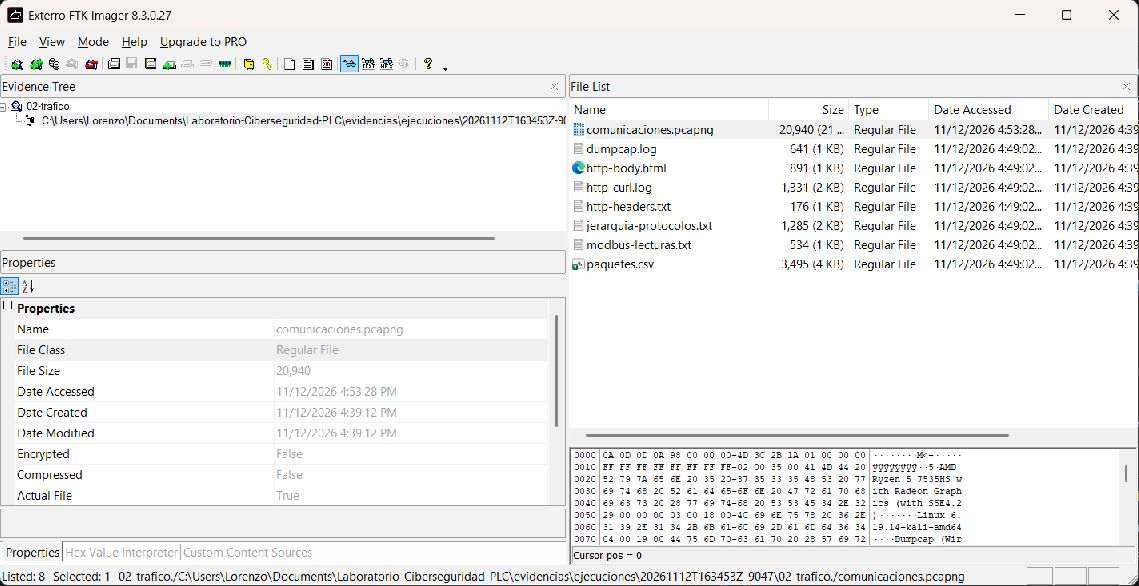
\includegraphics[width=0.78\linewidth]{07-ftk-inspeccion.jpg}\caption{Inspección del PCAP original: propiedades y contenido.}\end{figure}
\textbf{3. Contrastar la integridad.} Get-FileHash de Windows volvió a calcular el SHA-256 de ese archivo y coincidió con su referencia original. El cálculo corresponde a esa herramienta; FTK se utilizó para la inspección de archivos. No se creó una imagen física de un disco.

\clearpage\section*{8. Recomendaciones para mejorar la seguridad}\label{recomendaciones}

\par\begin{tabularx}{\linewidth}{@{}P{3.2cm}YY@{}}\toprule
Condición & Recomendación & Cómo corroborarla después\\\midrule
Credencial pública & Sustituir credenciales predeterminadas y retirar cuentas innecesarias. & Intentar la credencial anterior en el entorno autorizado: debe rechazarse.\\
Terminal Telnet & Retirar Telnet y usar SSH con autenticación adecuada. & Comprobar que TCP 23 ya no acepta conexiones y que la administración cifrada funciona.\\
HTTP legible & Usar HTTPS con certificados validados cuando se transmita información que requiera protección. & Verificar el canal TLS y evitar exponer datos sensibles por HTTP.\\
Modbus accesible a clientes de la red & Segmentar y permitir únicamente clientes autorizados; proteger el acceso a la red industrial. & Comprobar lectura desde el cliente permitido y bloqueo desde uno no autorizado.\\
Servicios innecesarios & Reducir servicios expuestos y actualizar componentes compatibles con la operación. & Repetir el inventario y contrastar los puertos con los servicios aprobados.\\\bottomrule
\end{tabularx}
Las medidas son propuestas; no se aplicaron a la víctima didáctica antes de las capturas. Se conservaron sus condiciones para poder repetir la demostración.
\textbf{Preparación de la sustentación.} Revisar la red; descubrir equipos; explorar puertos; iniciar captura; generar HTTP y Modbus; analizar solicitudes/respuestas; abrir y cerrar la sesión Telnet; revisar su PCAP; comparar hashes. La guía separada presenta estas órdenes una por una, con el resultado que se debe observar y una explicación breve para exponerlo.

\clearpage\section*{9. Conclusiones del trabajo}\label{conclusiones}

El reconocimiento identificó dos blancos activos y 30 puertos TCP abiertos en la víctima; el PLC respondió en los dos puertos examinados. Las capturas permitieron reconocer el establecimiento TCP, una solicitud/respuesta HTTP y tres lecturas Modbus de cuatro registros simulados.
La sesión Telnet confirmó acceso con la credencial pública y permitió consultar la identidad y el sistema. La captura específica conservó la información transmitida, mostrando por qué ocultar una contraseña en pantalla no protege su tránsito por la red.
La comparación SHA-256 mantuvo la fuente y detectó una modificación en una copia. Los resultados respaldan reducir servicios, gestionar credenciales, cifrar la administración y limitar el acceso a las comunicaciones industriales.
\textbf{Alcance.} La práctica se limitó a las máquinas virtuales autorizadas; no se ensayó escritura Modbus ni se validó un PLC físico. Las capturas de este informe corresponden a una nueva demostración del 17 de noviembre. Sus tramas, puertos dinámicos y hashes son propios de esa corrida; los resultados anteriores se conservan separados.
\textbf{Archivos de consulta.} El guion \texttt{docs/SUSTENTACION\_PASO\_A\_PASO.md} permite repetir las órdenes; \texttt{docs/MATRIZ\_CUMPLIMIENTO.md} relaciona los requisitos con estas secciones. Los archivos del laboratorio se conservan por corrida y tipo de evidencia.
\textbf{Referencias.}\par
{\small\raggedright
[1] Rapid7, \href{https://docs.rapid7.com/metasploit/metasploitable-2/}{Metasploitable 2}.\par
[2] MITRE, \href{https://cwe.mitre.org/data/definitions/1392.html}{CWE-1392: uso de credenciales predeterminadas}.\par
[3] MITRE, \href{https://cwe.mitre.org/data/definitions/319.html}{CWE-319: información sensible transmitida en claro}.\par
[4] MITRE, \href{https://www.mitre.org/who-we-are}{Who We Are}.\par
[5] CVE Program, \href{https://www.cve.org/Resources/Media/Archives/OldWebsite/index.html}{Descripción del programa CVE}.\par
[6] RFC Editor, \href{https://www.rfc-editor.org/rfc/rfc854}{RFC 854: Telnet Protocol Specification}.\par
Guía académica original de la Universidad Santo Tomás: actividades, nueve apartados y criterios de evaluación.\par}
\end{document}

